\section{Veränderungen}
\subsection{Klassendiagramm}
Im Folgenden wird anhand des Klassendiagramms aus der Entwurfsphase und eines aktualisierten Klassendiagramms gezeigt, was sich zum Entwurf verändert hat.

\begin{figure}[H]
	\centering
	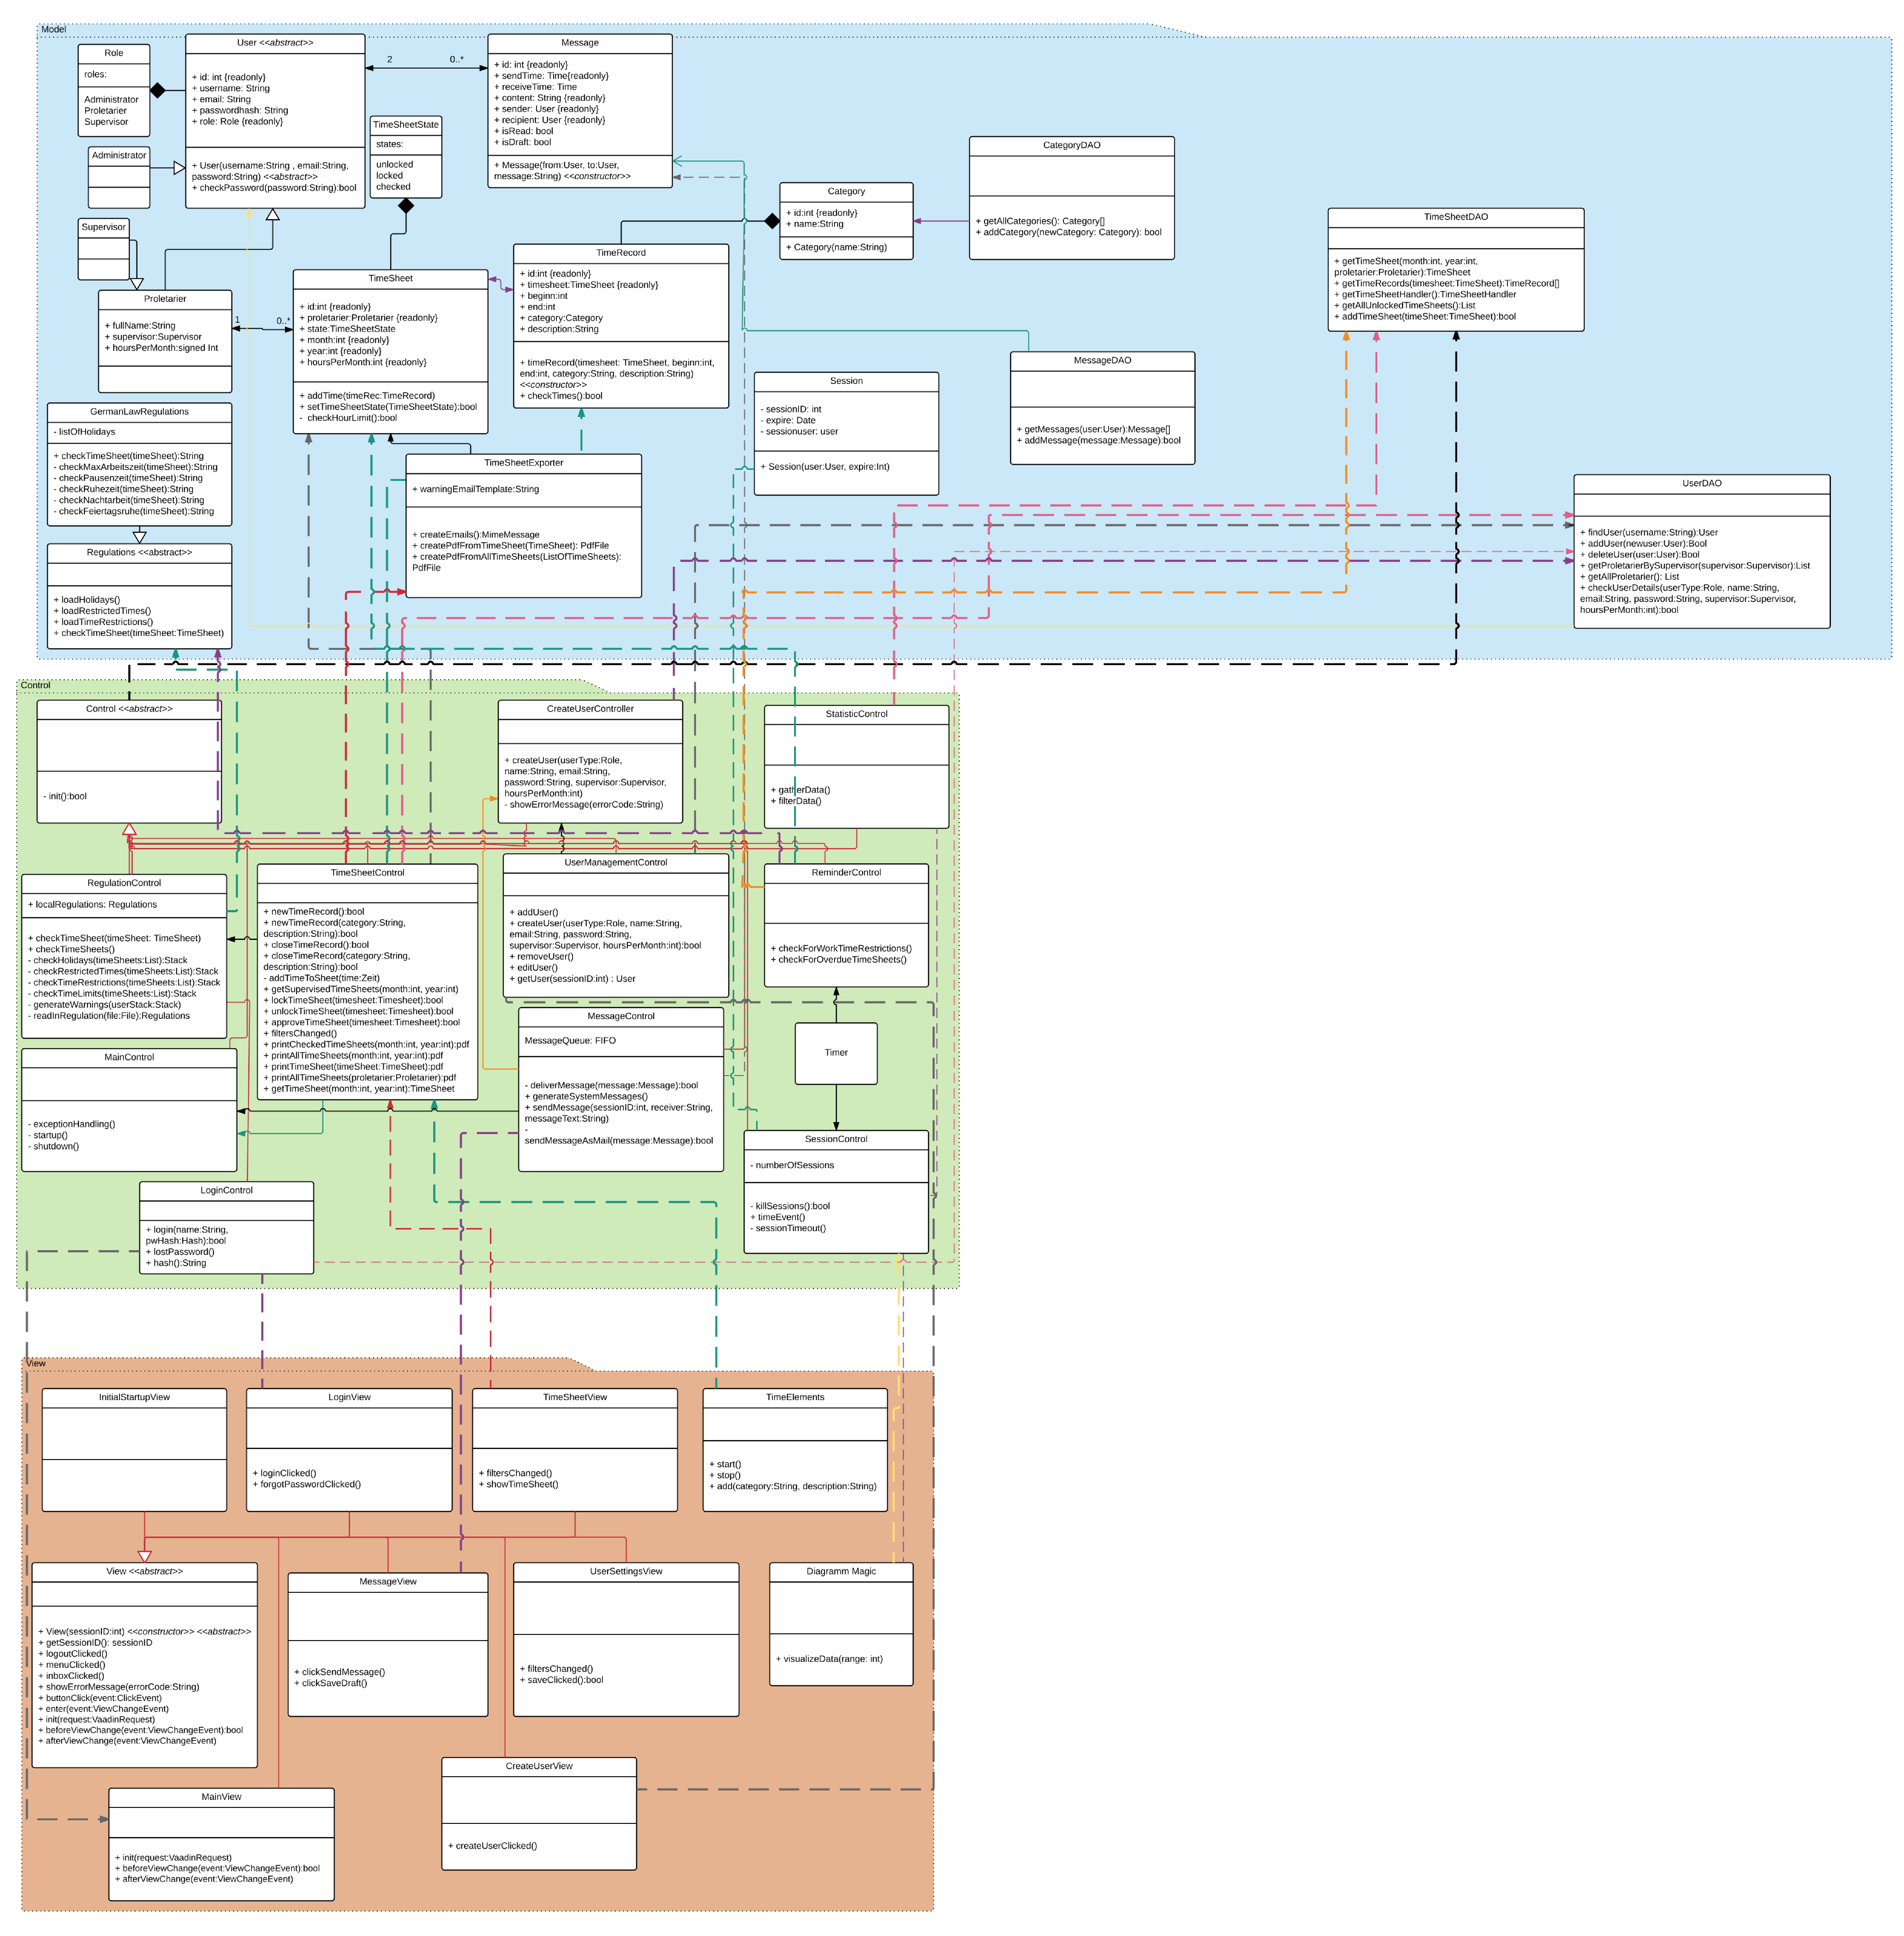
\includegraphics[scale=0.135]{Class-Diagramm_alt.pdf}
	\caption{Altes Klassendiagramm}
\end{figure}
\newpage

In der view haben sich folgenden Änderungen ergeben:
\VerbatimInput[fontsize=\small]{view-diff}

Die meisten Änderungen in der \emph{View} sind durch Vaadin entstanden. 
Im speziellen mussten Methoden und Attribute angepasst oder hinzugefügt werden, 
damit \emph{Vaadin} funktioniert.
Es wurden auch drei neue Sichten hinzugefügt, \emph{AdminView}, \emph{SupervisorView} und \emph{TimeRecordView}, 
dafür wurde auch das Packet \emph{view.forms} erstellt.
Die abstrakte \emph{View} wurde gelöscht, da mit \emph{Vaadin} das gewünschte Entwurfsmuster 
ohne weitere Aufwendungen nicht umsetzbar war.
Die \emph{MessageView} wurde entfernt aufgrund einer Änderung der Anforderungen an das Projekt.\\
\\
In der control haben sich folgende Änderungen ergeben:
\VerbatimInput[fontsize=\small]{control-diff}

Wie auch zuerst in der \emph{View} angedacht, wurde auch in der \emph{Control} die abstrakte \emph{Control} Klasse 
nicht wie beabsichtigt angewendet werden.
Es wurden zwei neue Klassen erstellt, welche für den \emph{Scheduler} benötigt werden. 
Die Klasse \emph{Timer} wurde zu \emph{SchedulerHandler} umbenannt, damit der Name besser zur Funktionalität passt.
Die Methoden aus der \emph{ReminderControl} wurden in das \emph{Model} verschoben.
Weitere Methoden mussten unter anderem zur \emph{UserManagementControl} und \emph{TimeSheetControl} hinzugefügt werden, 
um andere Funktionalitäten und Änderungen im \emph{Backend} korrekt zu unterstützen.\\
\\
Im model haben sich folgende Änderungen ergeben:
\VerbatimInput[fontsize=\small]{model-diff}

Die drei Rollen \emph{Proletarier}, \emph{Supervisor} und \emph{Administrator} wurden gelöscht, da durch 
die Änderung von \emph{Role} von Enum zu Klasse, sie unnötig wurden. Die Klasse \emph{UserDAO} wurde ebenso gelöscht.
\emph{Message} wurde zu Enum, da die Anforderungen sich geändert haben und 
die Klasse mit ursprünglicher Funktionalität nicht mehr nötig ist. Mit dazu wird auch die Klasse \emph{MessageDAO} nicht mehr benötigt.
Wir können auch die Klasse \emph{Session} löschen, da die Verwaltung von Sessions komplett von \emph{Shiro} Äbernommen wird.
Im \emph{TimeSheetDAO} wurden, vorallem zur \emph{TimeSheetControl}, passende Methoden hinzugefügt.
Von der gelöschten \emph{Proletarier} Klasse wurden die Methoden in \emph{User} verschoben.
Zur Unterstützung der DAO Klassen wurde zusätlich die Klasse \emph{DAOHelper} implementiert.\\
\\
Neu hinzugekommen ist security:
\VerbatimInput[fontsize=\small]{security-diff}

Security wurde durch die Verwendung von Shiro benötigt und wird deshalb auch in das Klassendiagramm aufgenommen.
\newpage

Daraus ergibt sich das aktualisierte Klassendiagramm:

\begin{figure}[H]
	\centering
	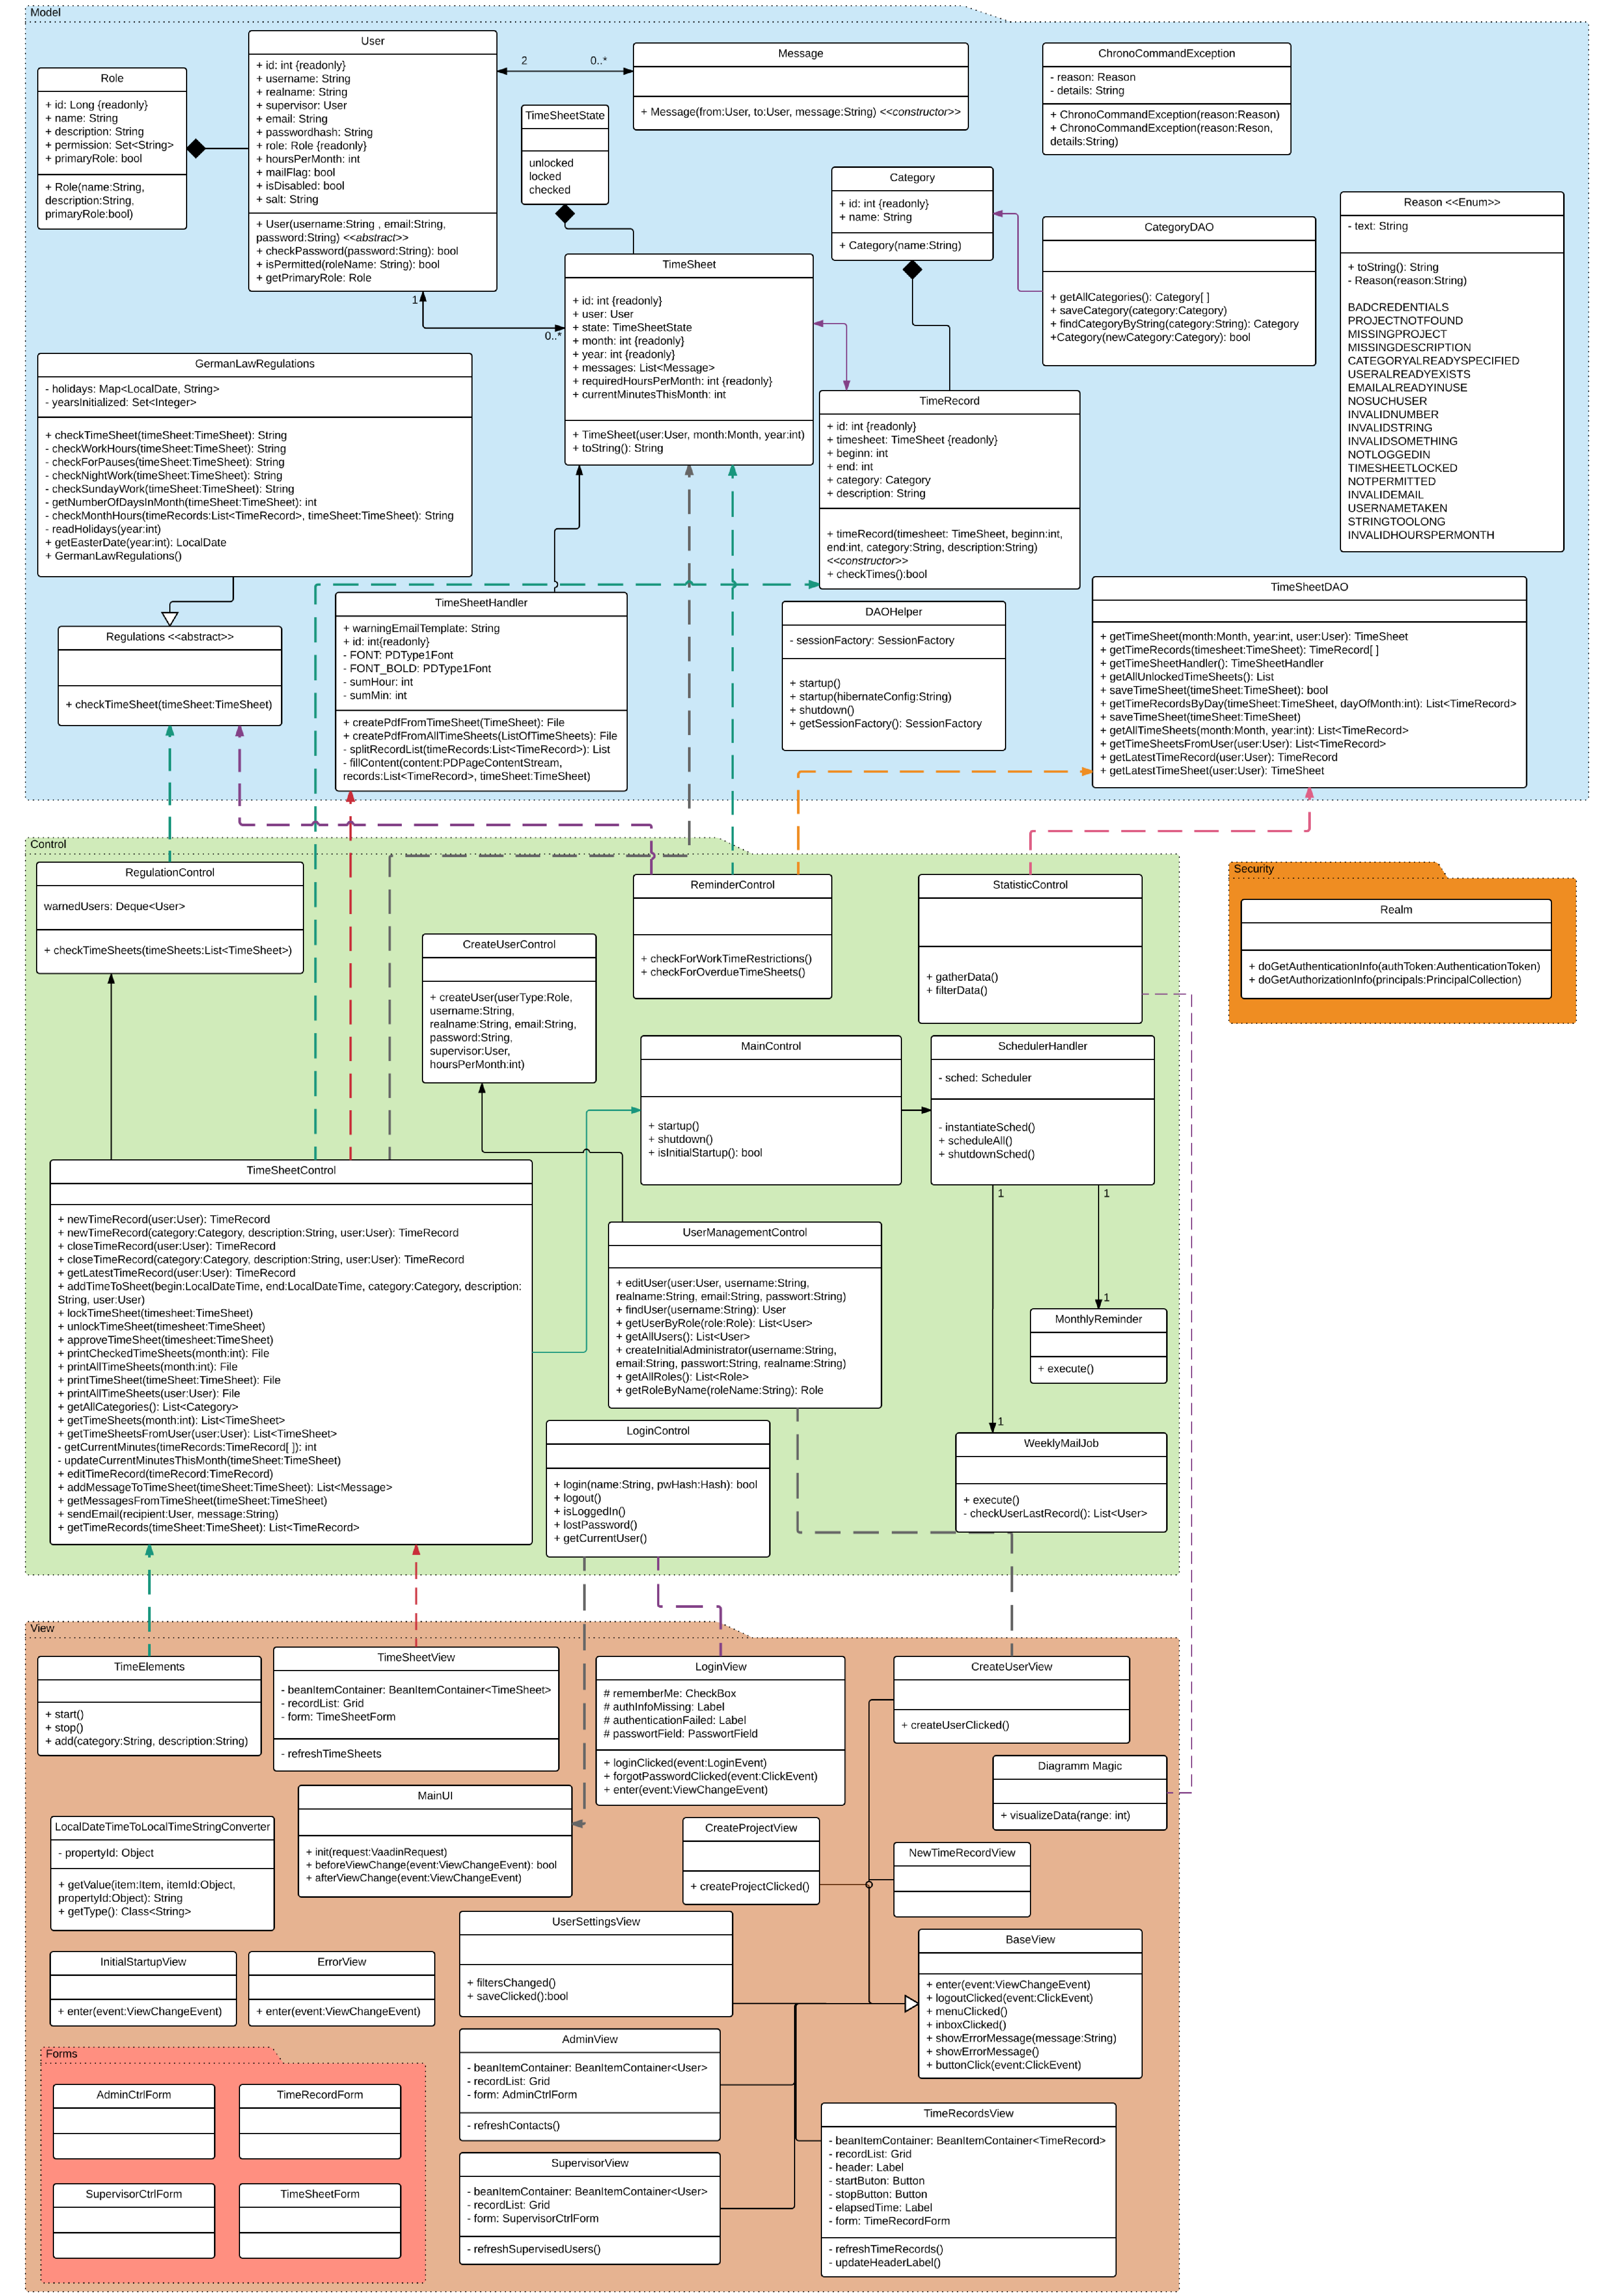
\includegraphics[scale=0.17]{Class-Diagramm-new.pdf}
	\caption{Neues Klassendiagramm}
\end{figure}
\newpage

\subsection{Sequenzen}
Die Sequenzdiagramme aus dem Entwurfen haben sich wie folgt verändert:
\subsubsection{Login Sequenz}

\begin{figure}[H]
      \centering
        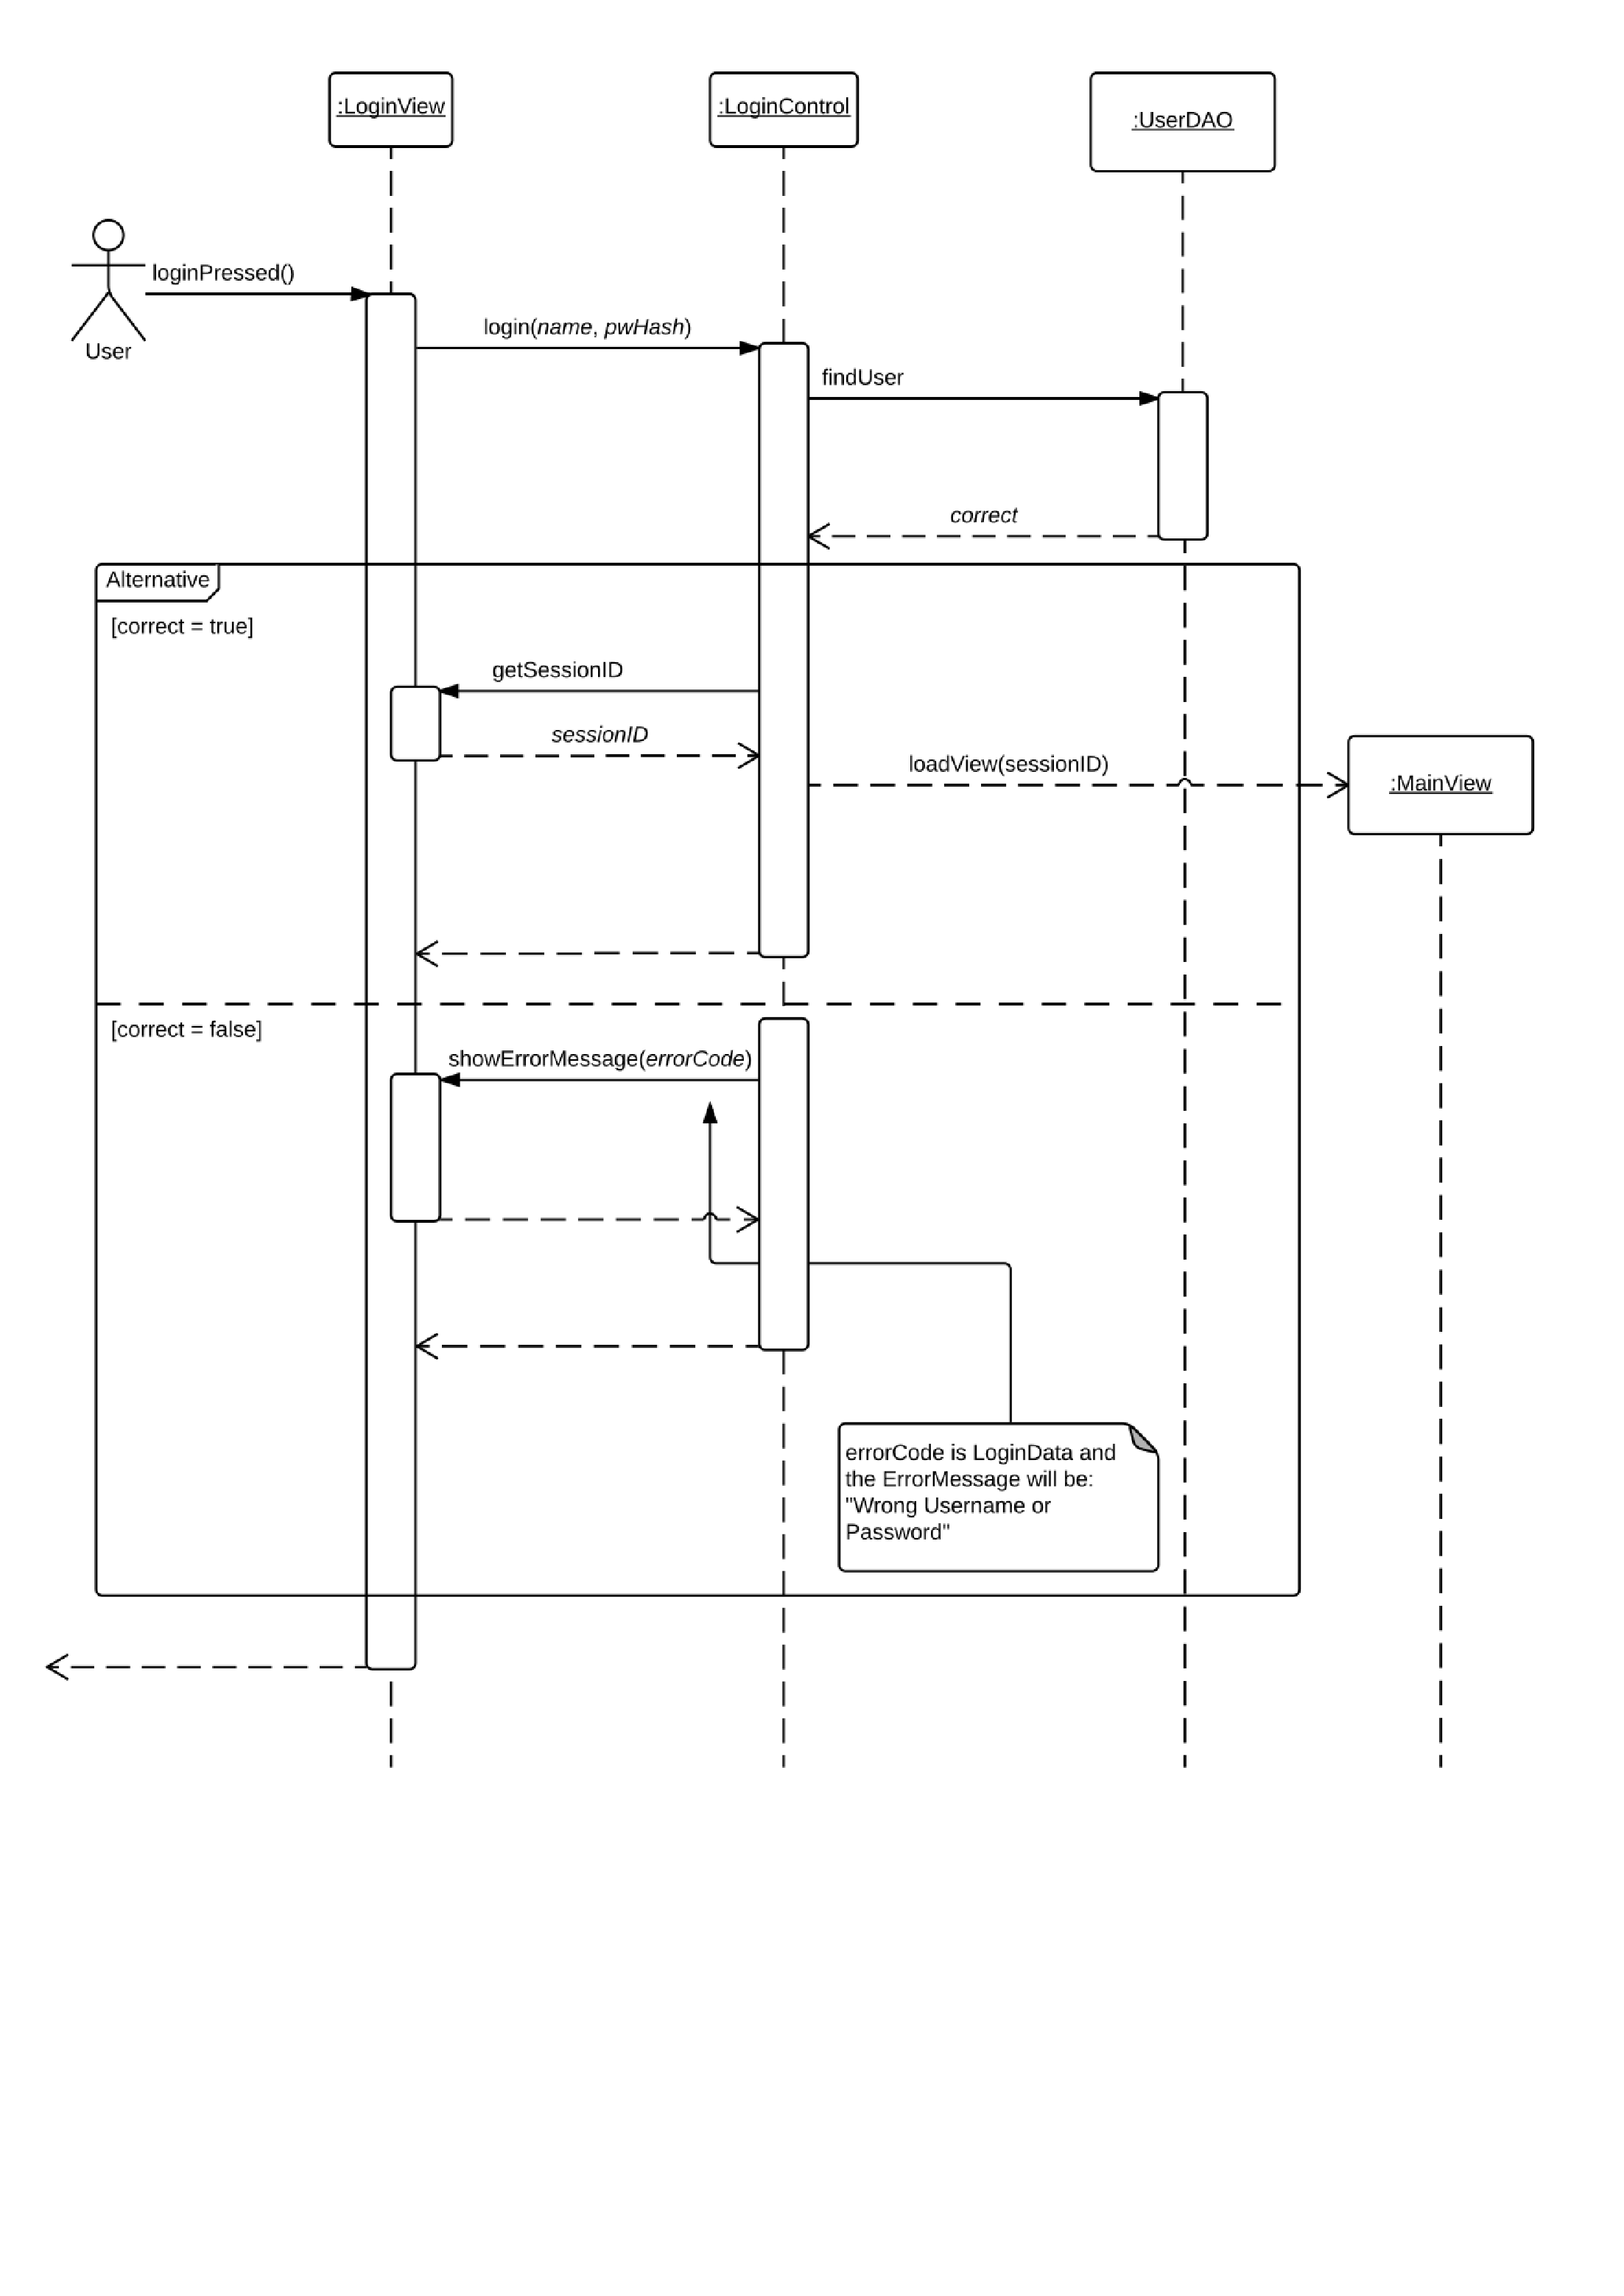
\includegraphics[scale=0.1]{Login-Sequenz.pdf}
       \caption{Alte Login Sequenz}
    \end{figure}

    \paragraph{Veränderungen}
        \begin{itemize}
            \item Login wurde um die Funktion \emph{remember me} erweitert.
            \item Die Authentifizierung wurde in einklang mit dem Shiro Framework gestaltet:
            \begin{itemize}
                \item Zum Login wird ein token aus Passwort und Username genutzt.
                \item Durch das Token wird der Nutzer ermittelt und dessen Authentifizierungsdaten (Password, ...) geholt.
                \item Diese werden mittels einen speziellen Hash vergleicher mit dem angegebenen Token verglichen.
            \end{itemize}
            \item Laden der View wurde durch Vaadins \emph{navigateTo} ersetzt.
        \end{itemize}

    \begin{figure}[H]
      \centering
        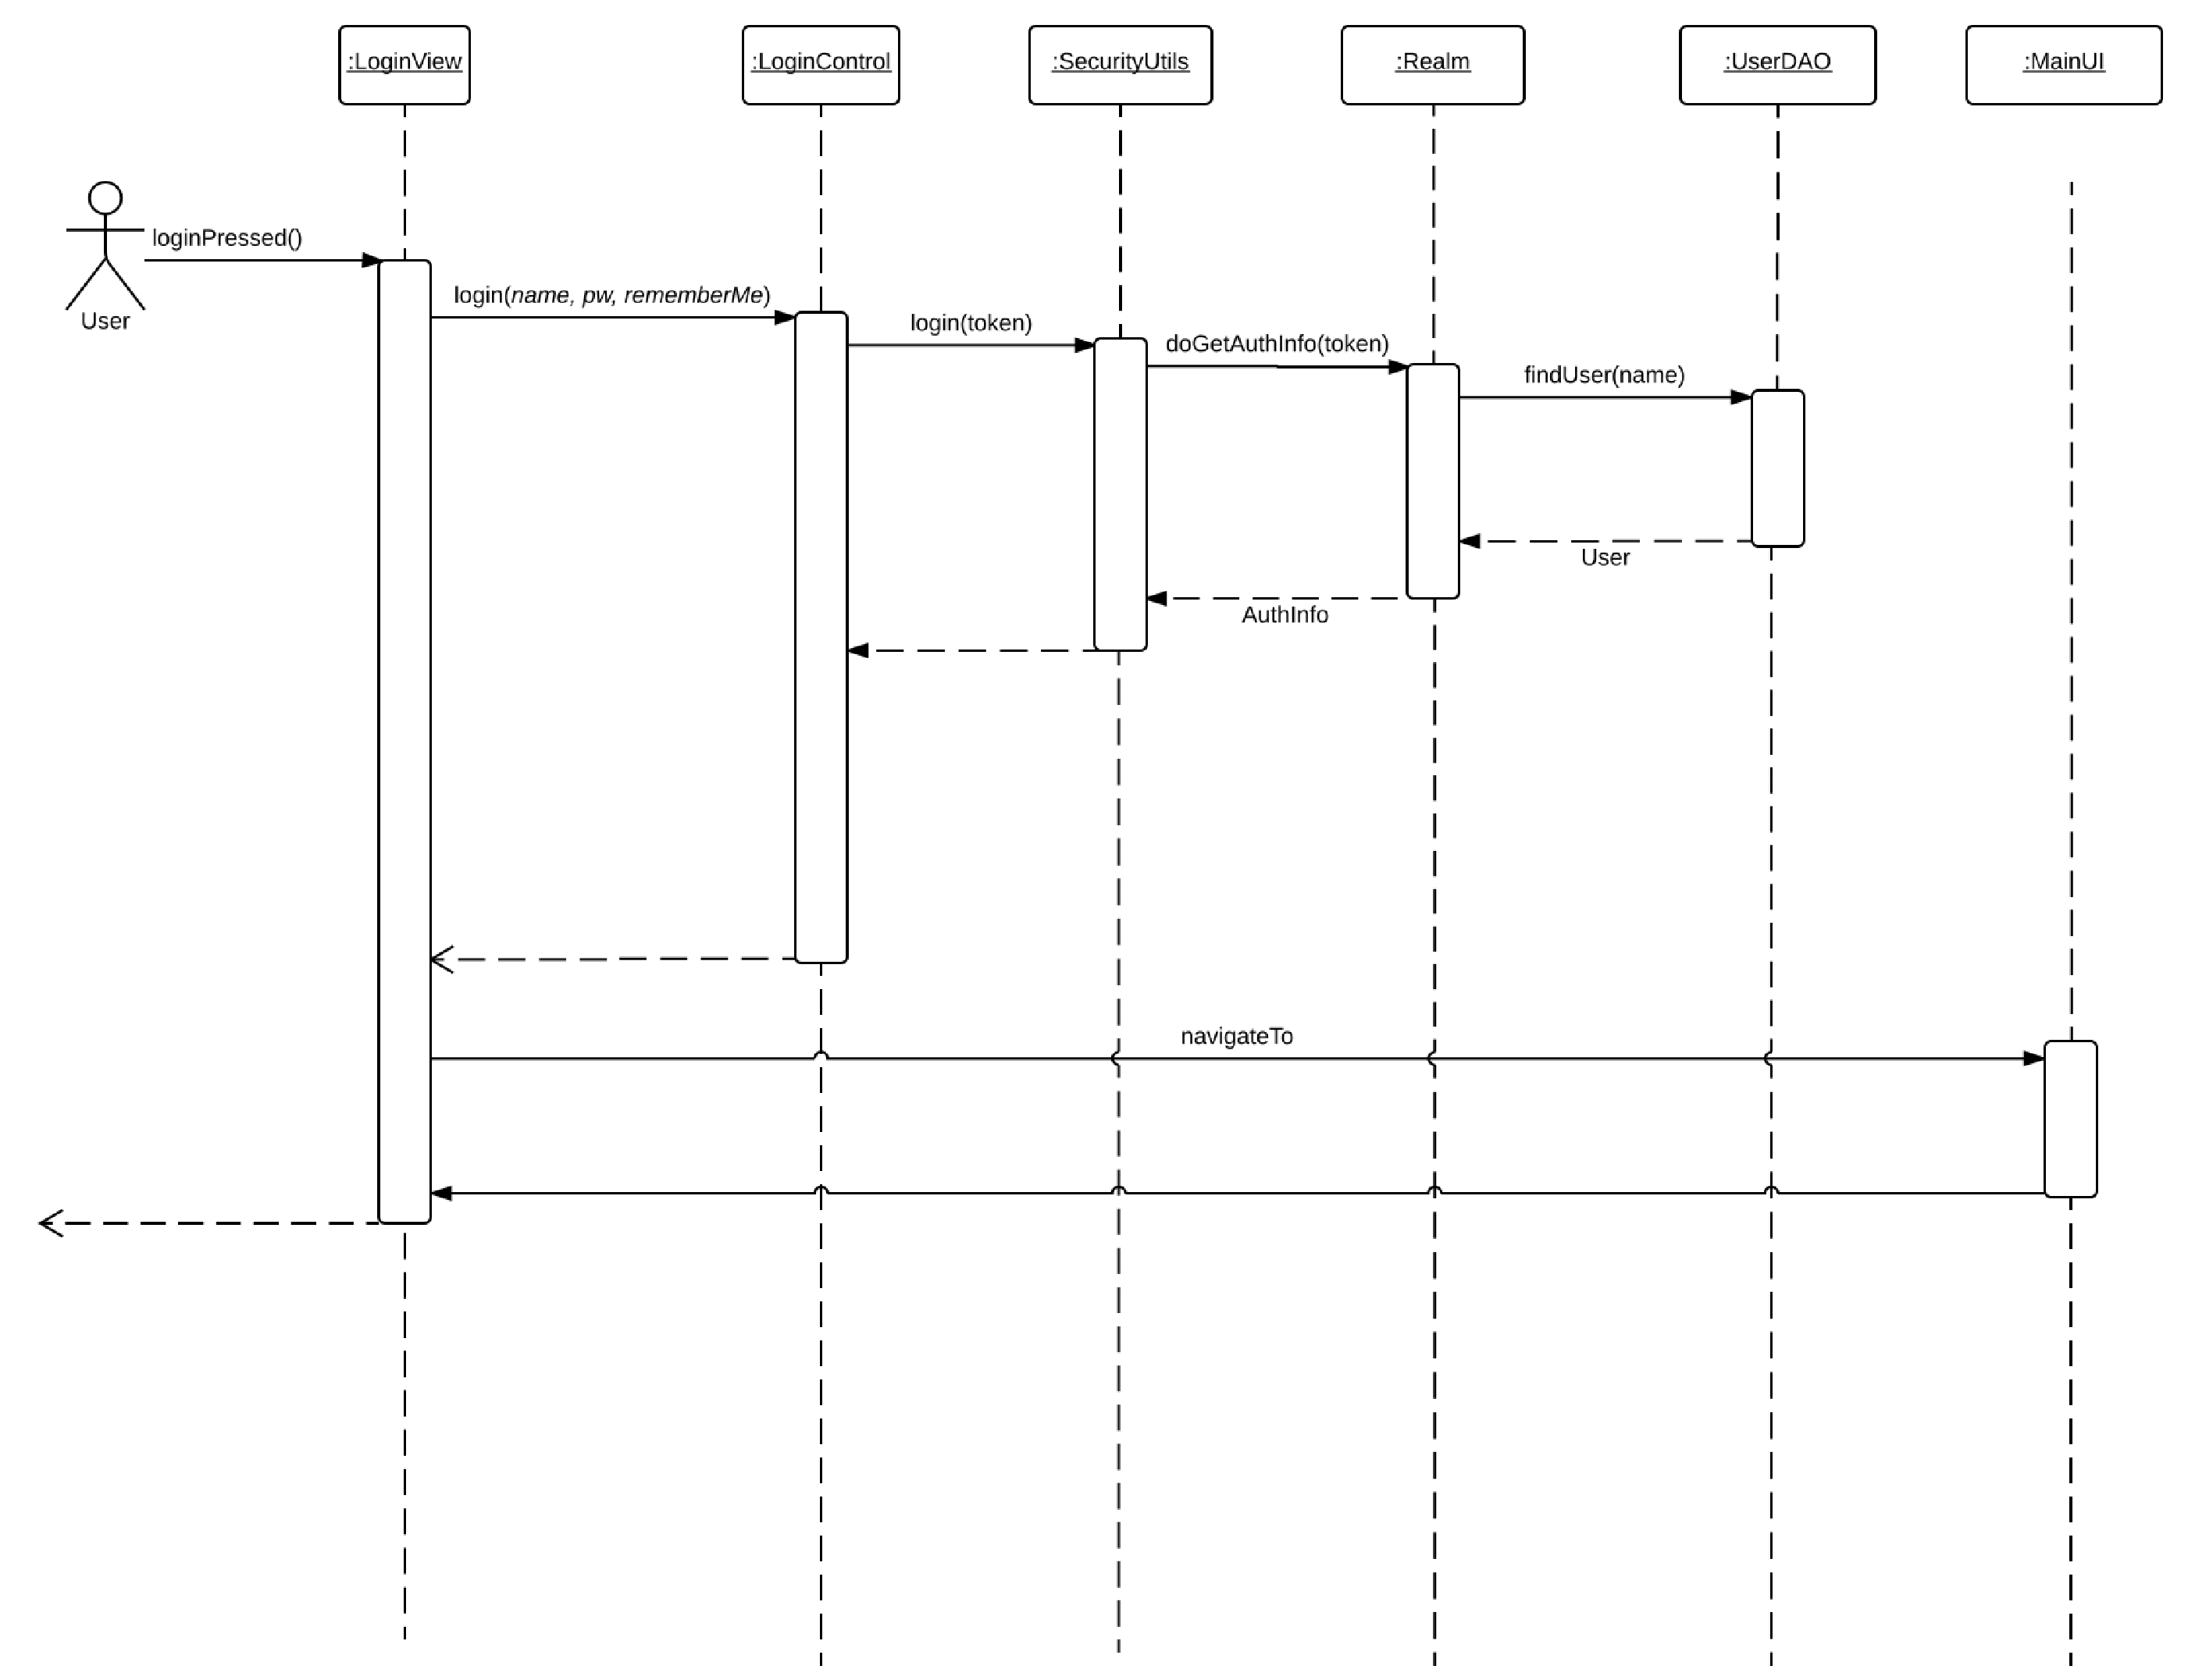
\includegraphics[scale=0.1]{Login-Sequenz-new.pdf}
       \caption{Neue Login Sequenz}
    \end{figure}

    \newpage
    \subsubsection{Account erstellungs Sequenz}

    \begin{figure}[H]
      \centering
        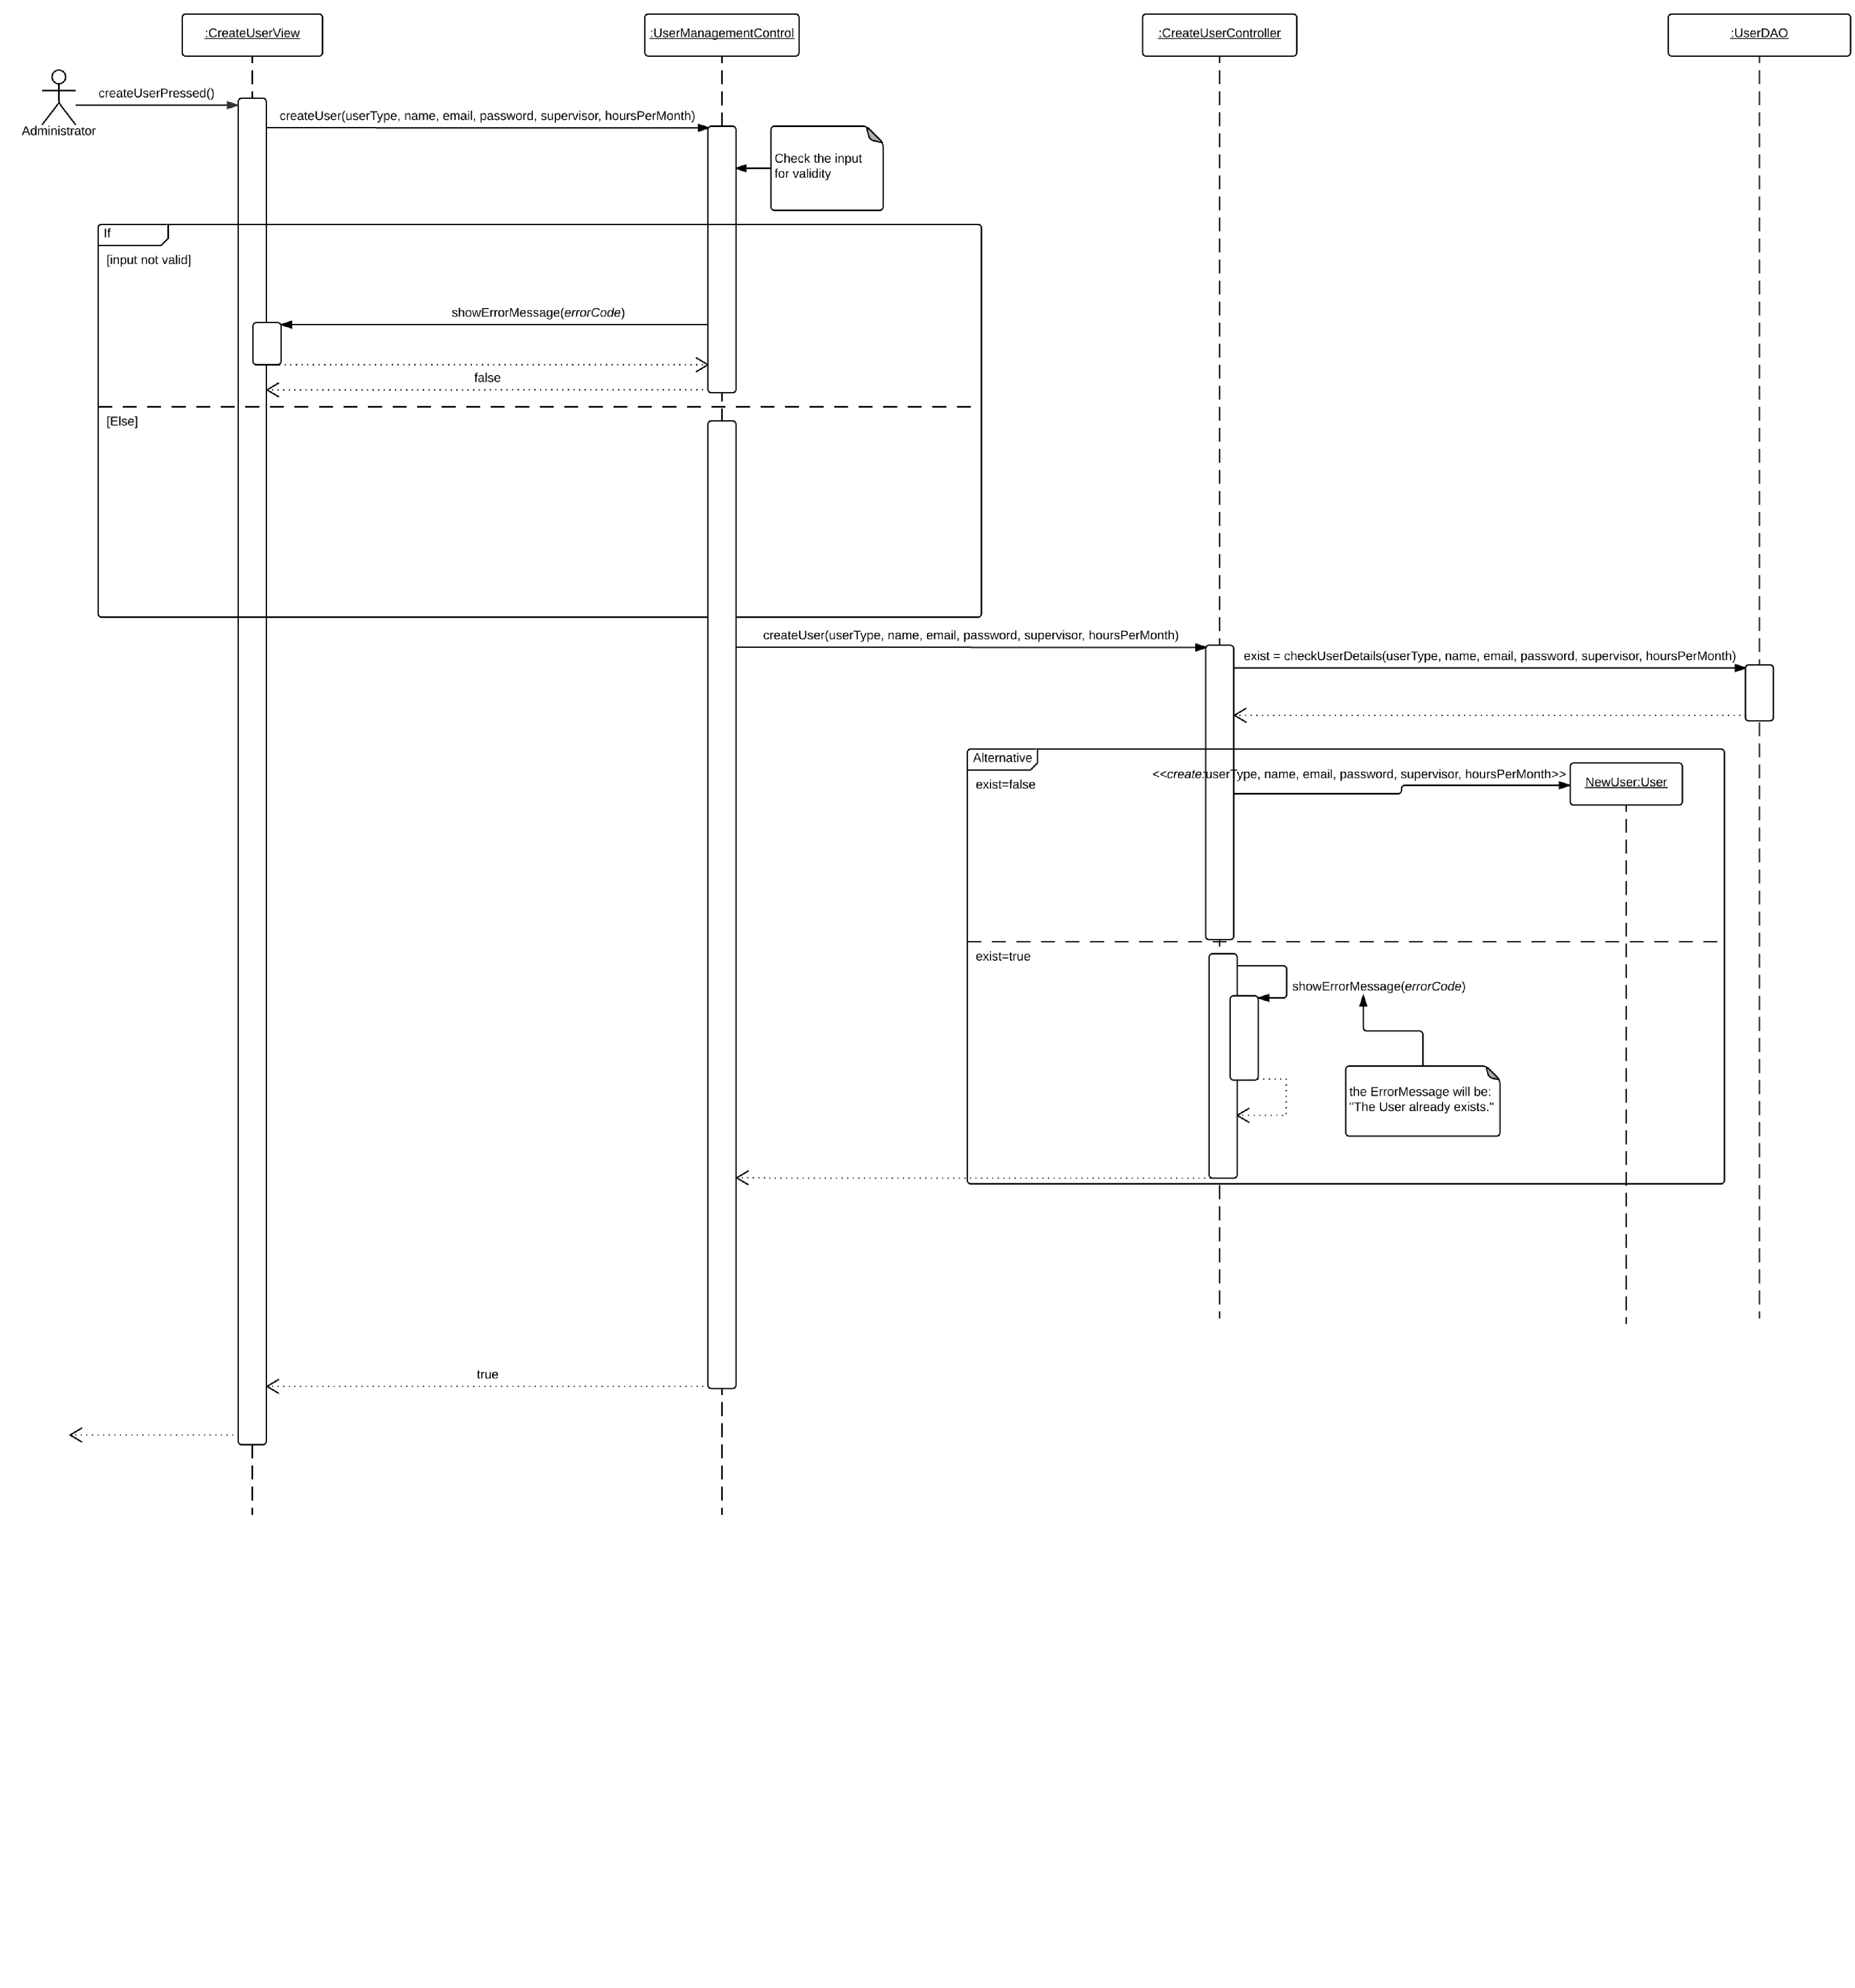
\includegraphics[scale=0.1]{Create-user-account.pdf}
       \caption{alte Benutzererstellungssequenz}
    \end{figure}

    \paragraph{Veränderungen}
        \begin{itemize}
            \item Der Ablauf wurde vereinfacht. Es wird nurnoch die CreateUserControl Klasse angespochen.
            \item Überprüfungen wurden durch eine verbesserte klarere interne Exception Struktur vereinfacht.
        \end{itemize}

    \begin{figure}[H]
      \centering
        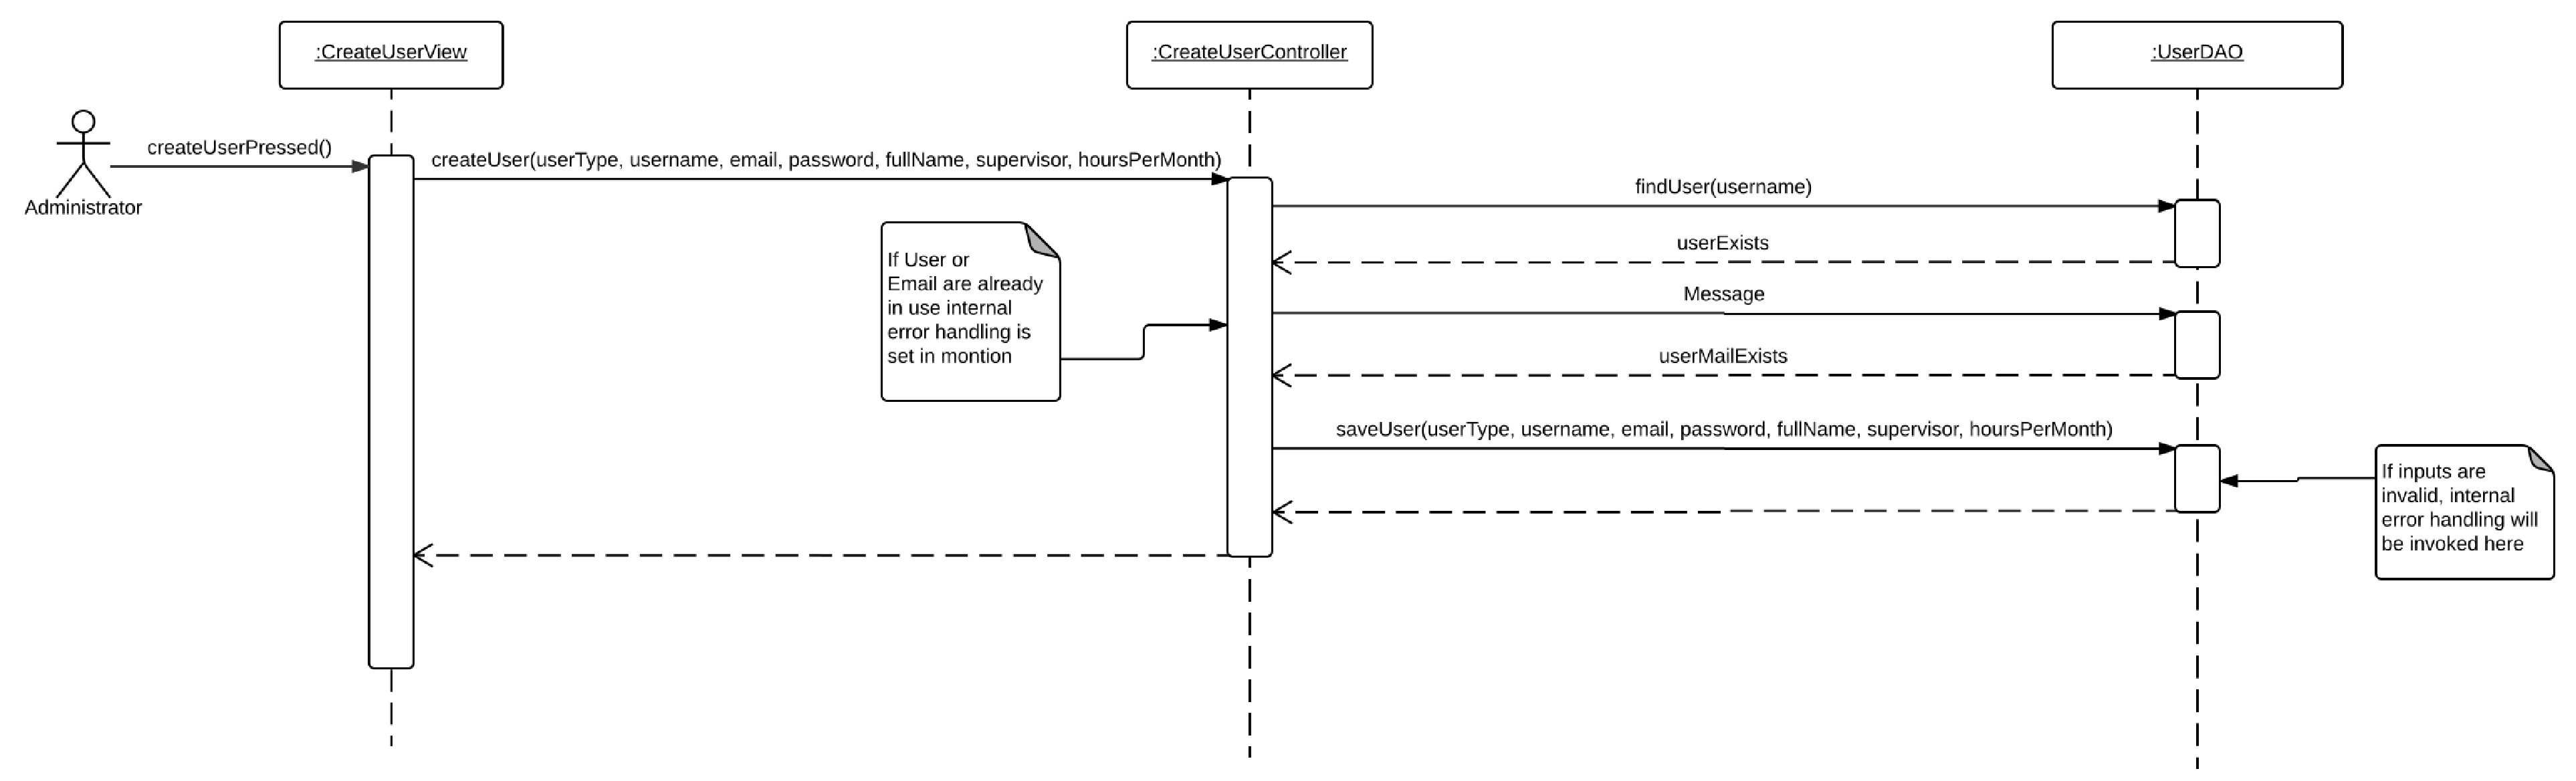
\includegraphics[scale=0.1]{Create-user-account-new.pdf}
       \caption{Neue Benutzererstellungssequenz}
    \end{figure}

    \newpage
\subsubsection{Neue Zeiterfassung - Sequenz}

    \begin{figure}[H]
      \centering
        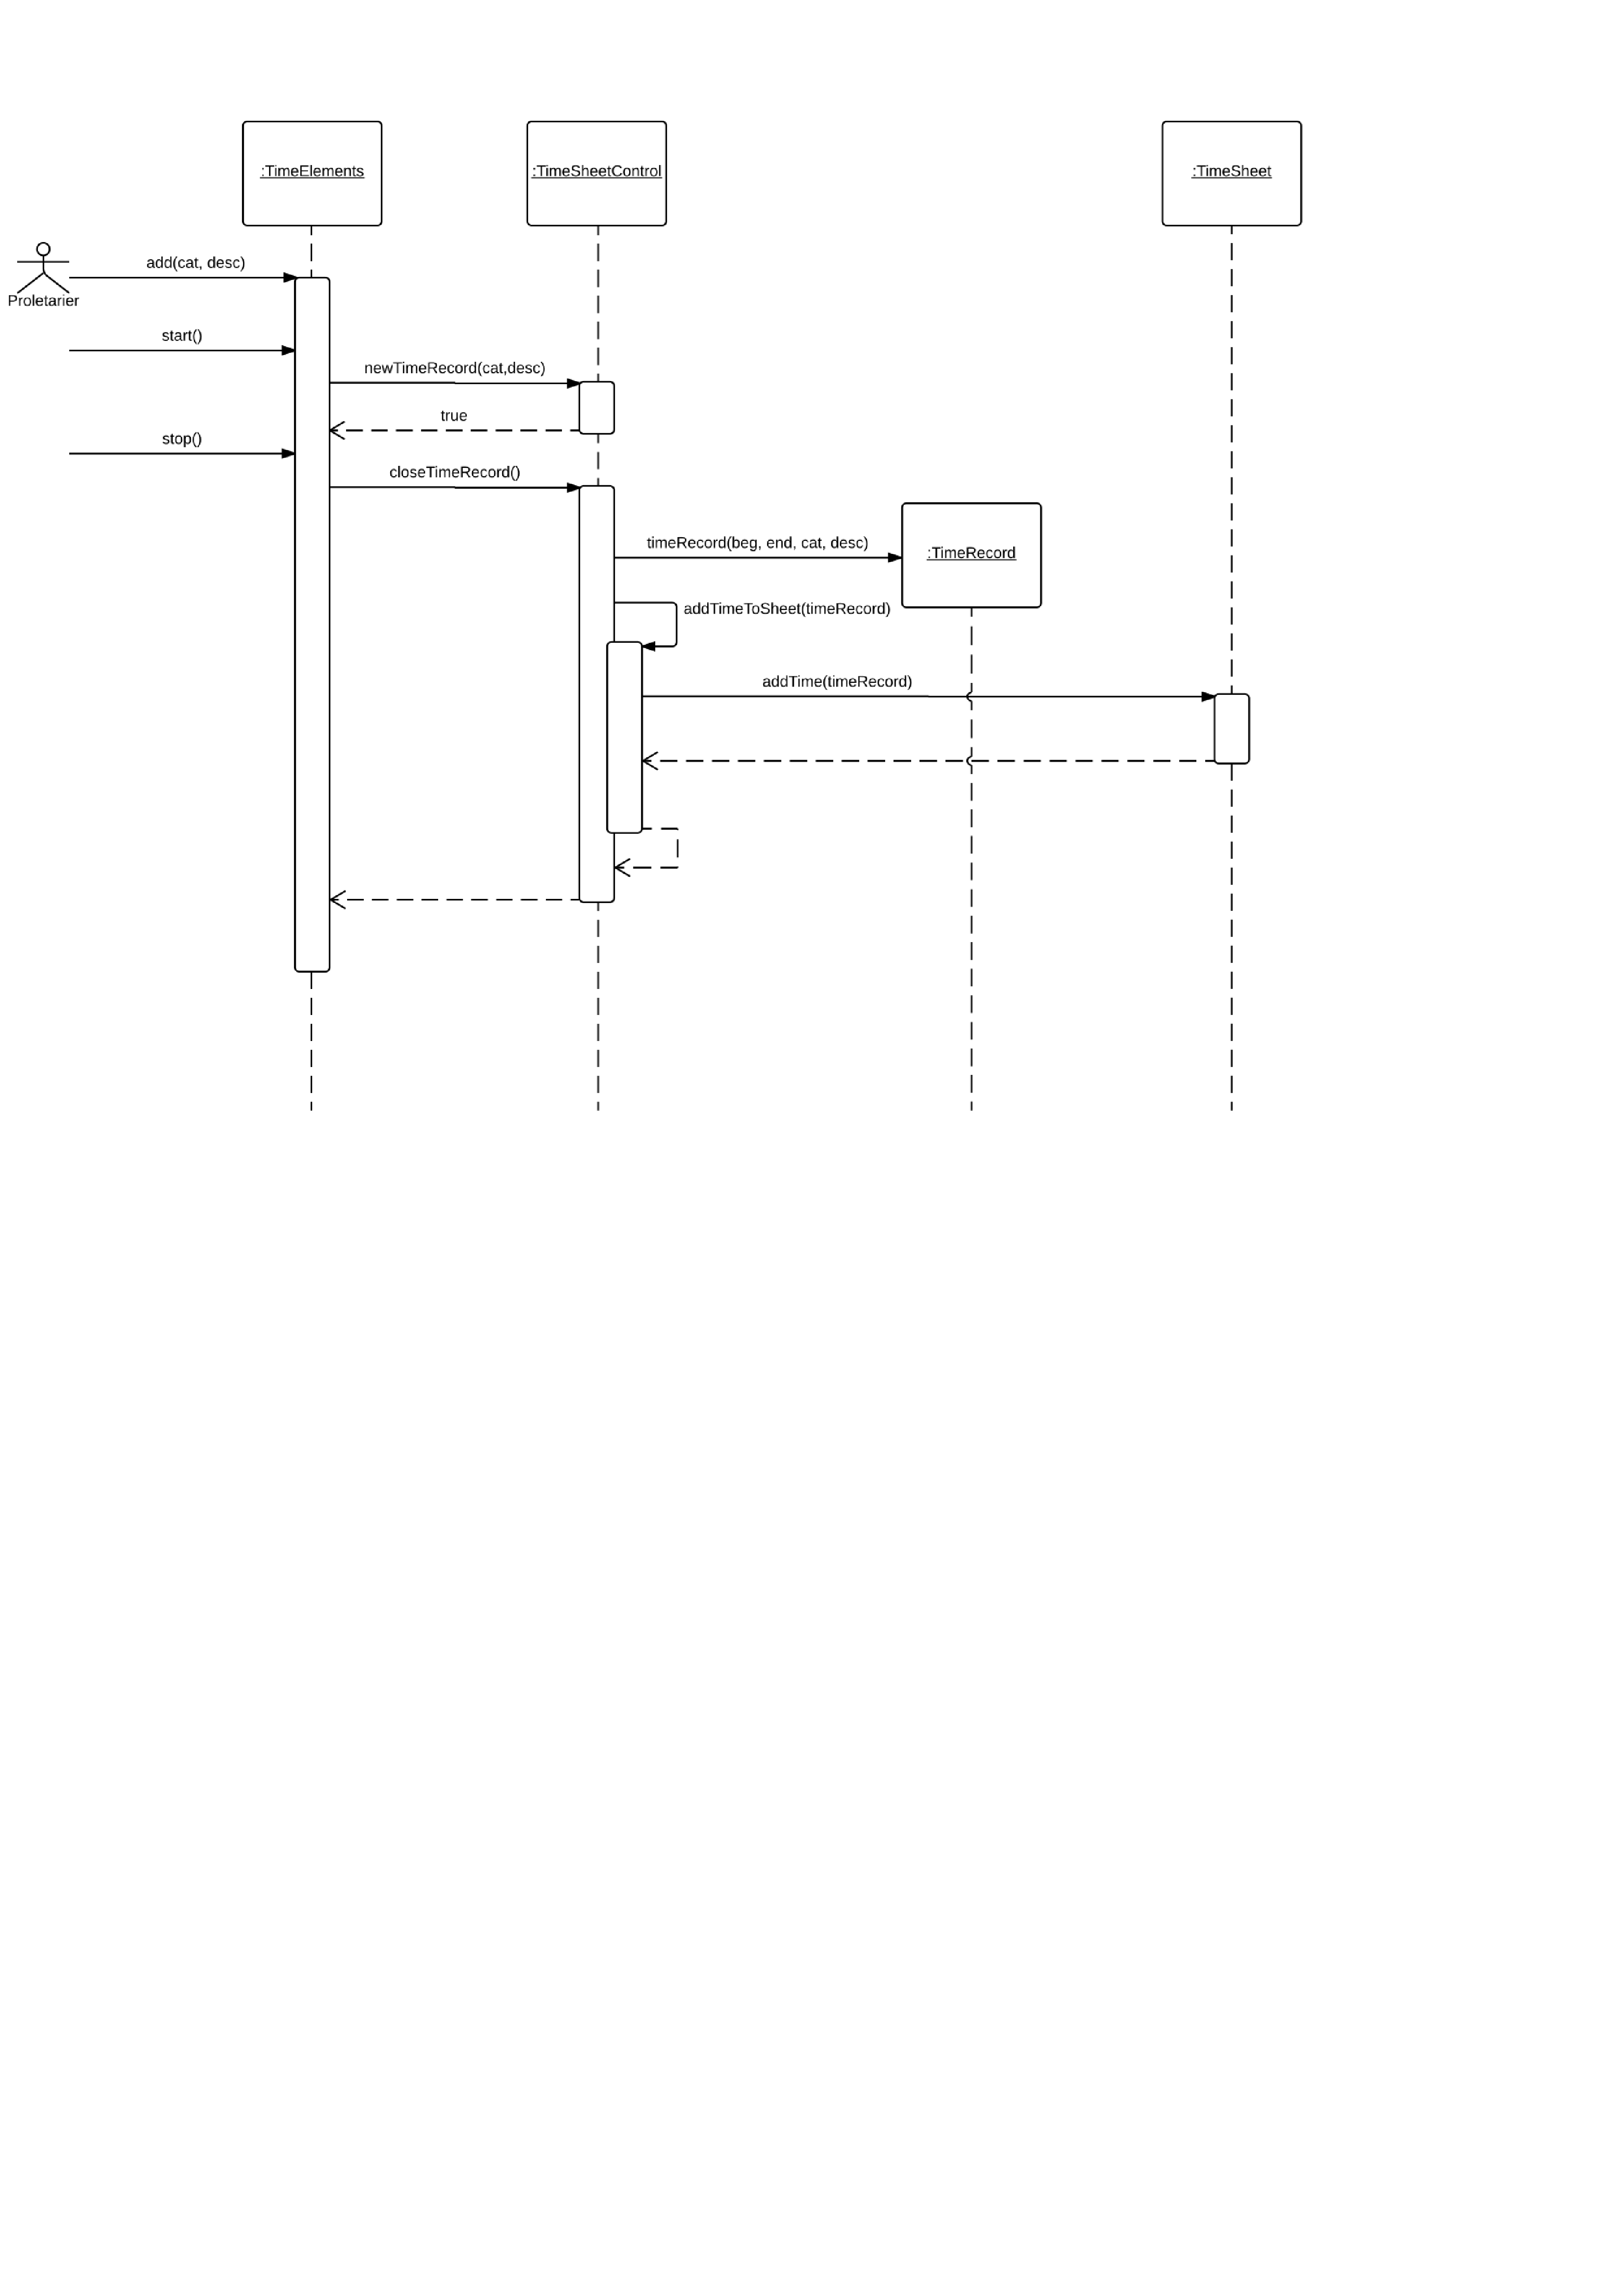
\includegraphics[scale=0.1]{new-Time-record.pdf}
       \caption{Alte Zeiterfassungssequenz}
    \end{figure}

    \paragraph{Veränderungen}
    \begin{itemize}
        \item Der Ablauf wurde in einklag mit Hibernate gebracht.
        \begin{itemize}
            \item Die TimeSheetControl kommuniziert nurnoch mit dem TimeSheetDAO
            \item TimeRecords werden erstellt und gespeichert, sobald die Zeiterfassung gestartet wurde (erhöhte persistenz)
            \item Wird der Tiem record geschlossen wird an dem jüngsten TimeRecord eine Endzeit hinzugefügt.
        \end{itemize}
        \item Das durchreichen von Wahrheitswerten wurde durch internes error handling ersetzt.
    \end{itemize}

    \begin{figure}[H]
      \centering
        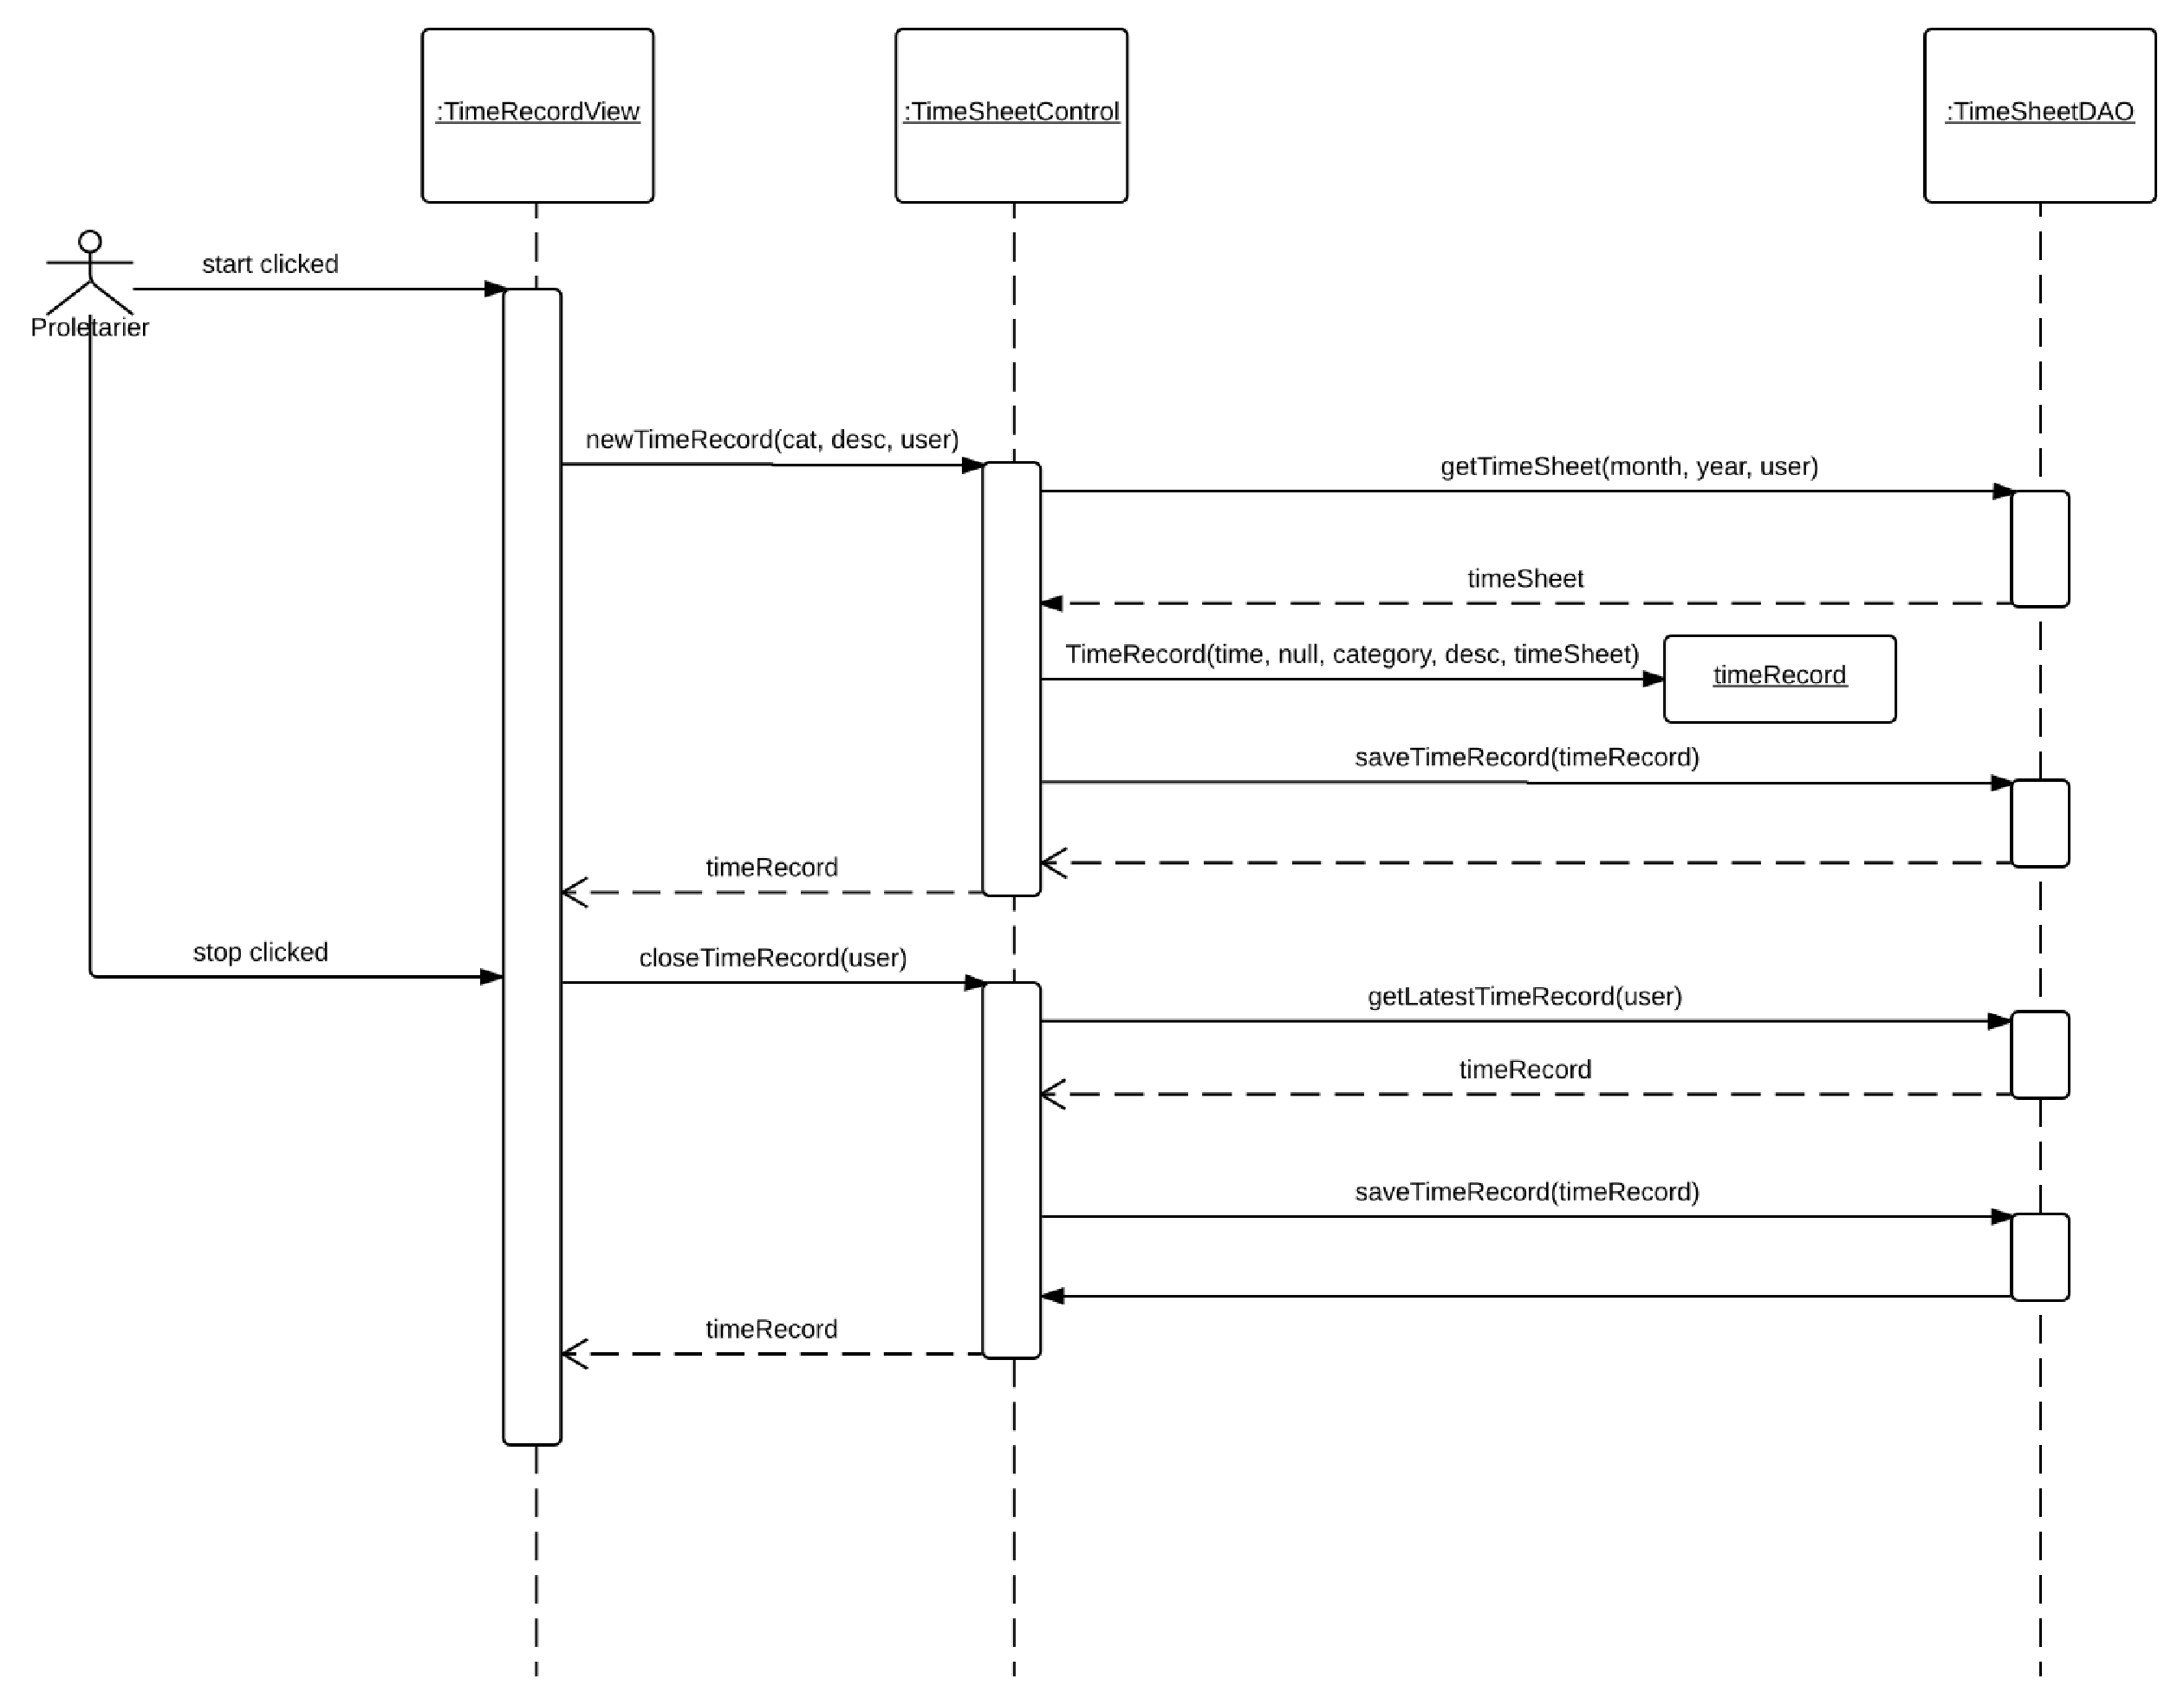
\includegraphics[scale=0.1]{new-Time-record-new.pdf}
       \caption{Neue Zeiterfassungssequenz}
    \end{figure}

    \newpage
\subsubsection{Admin druckt alle Stundenzettel - Sequenz}
    \begin{figure}[H]
      \centering
        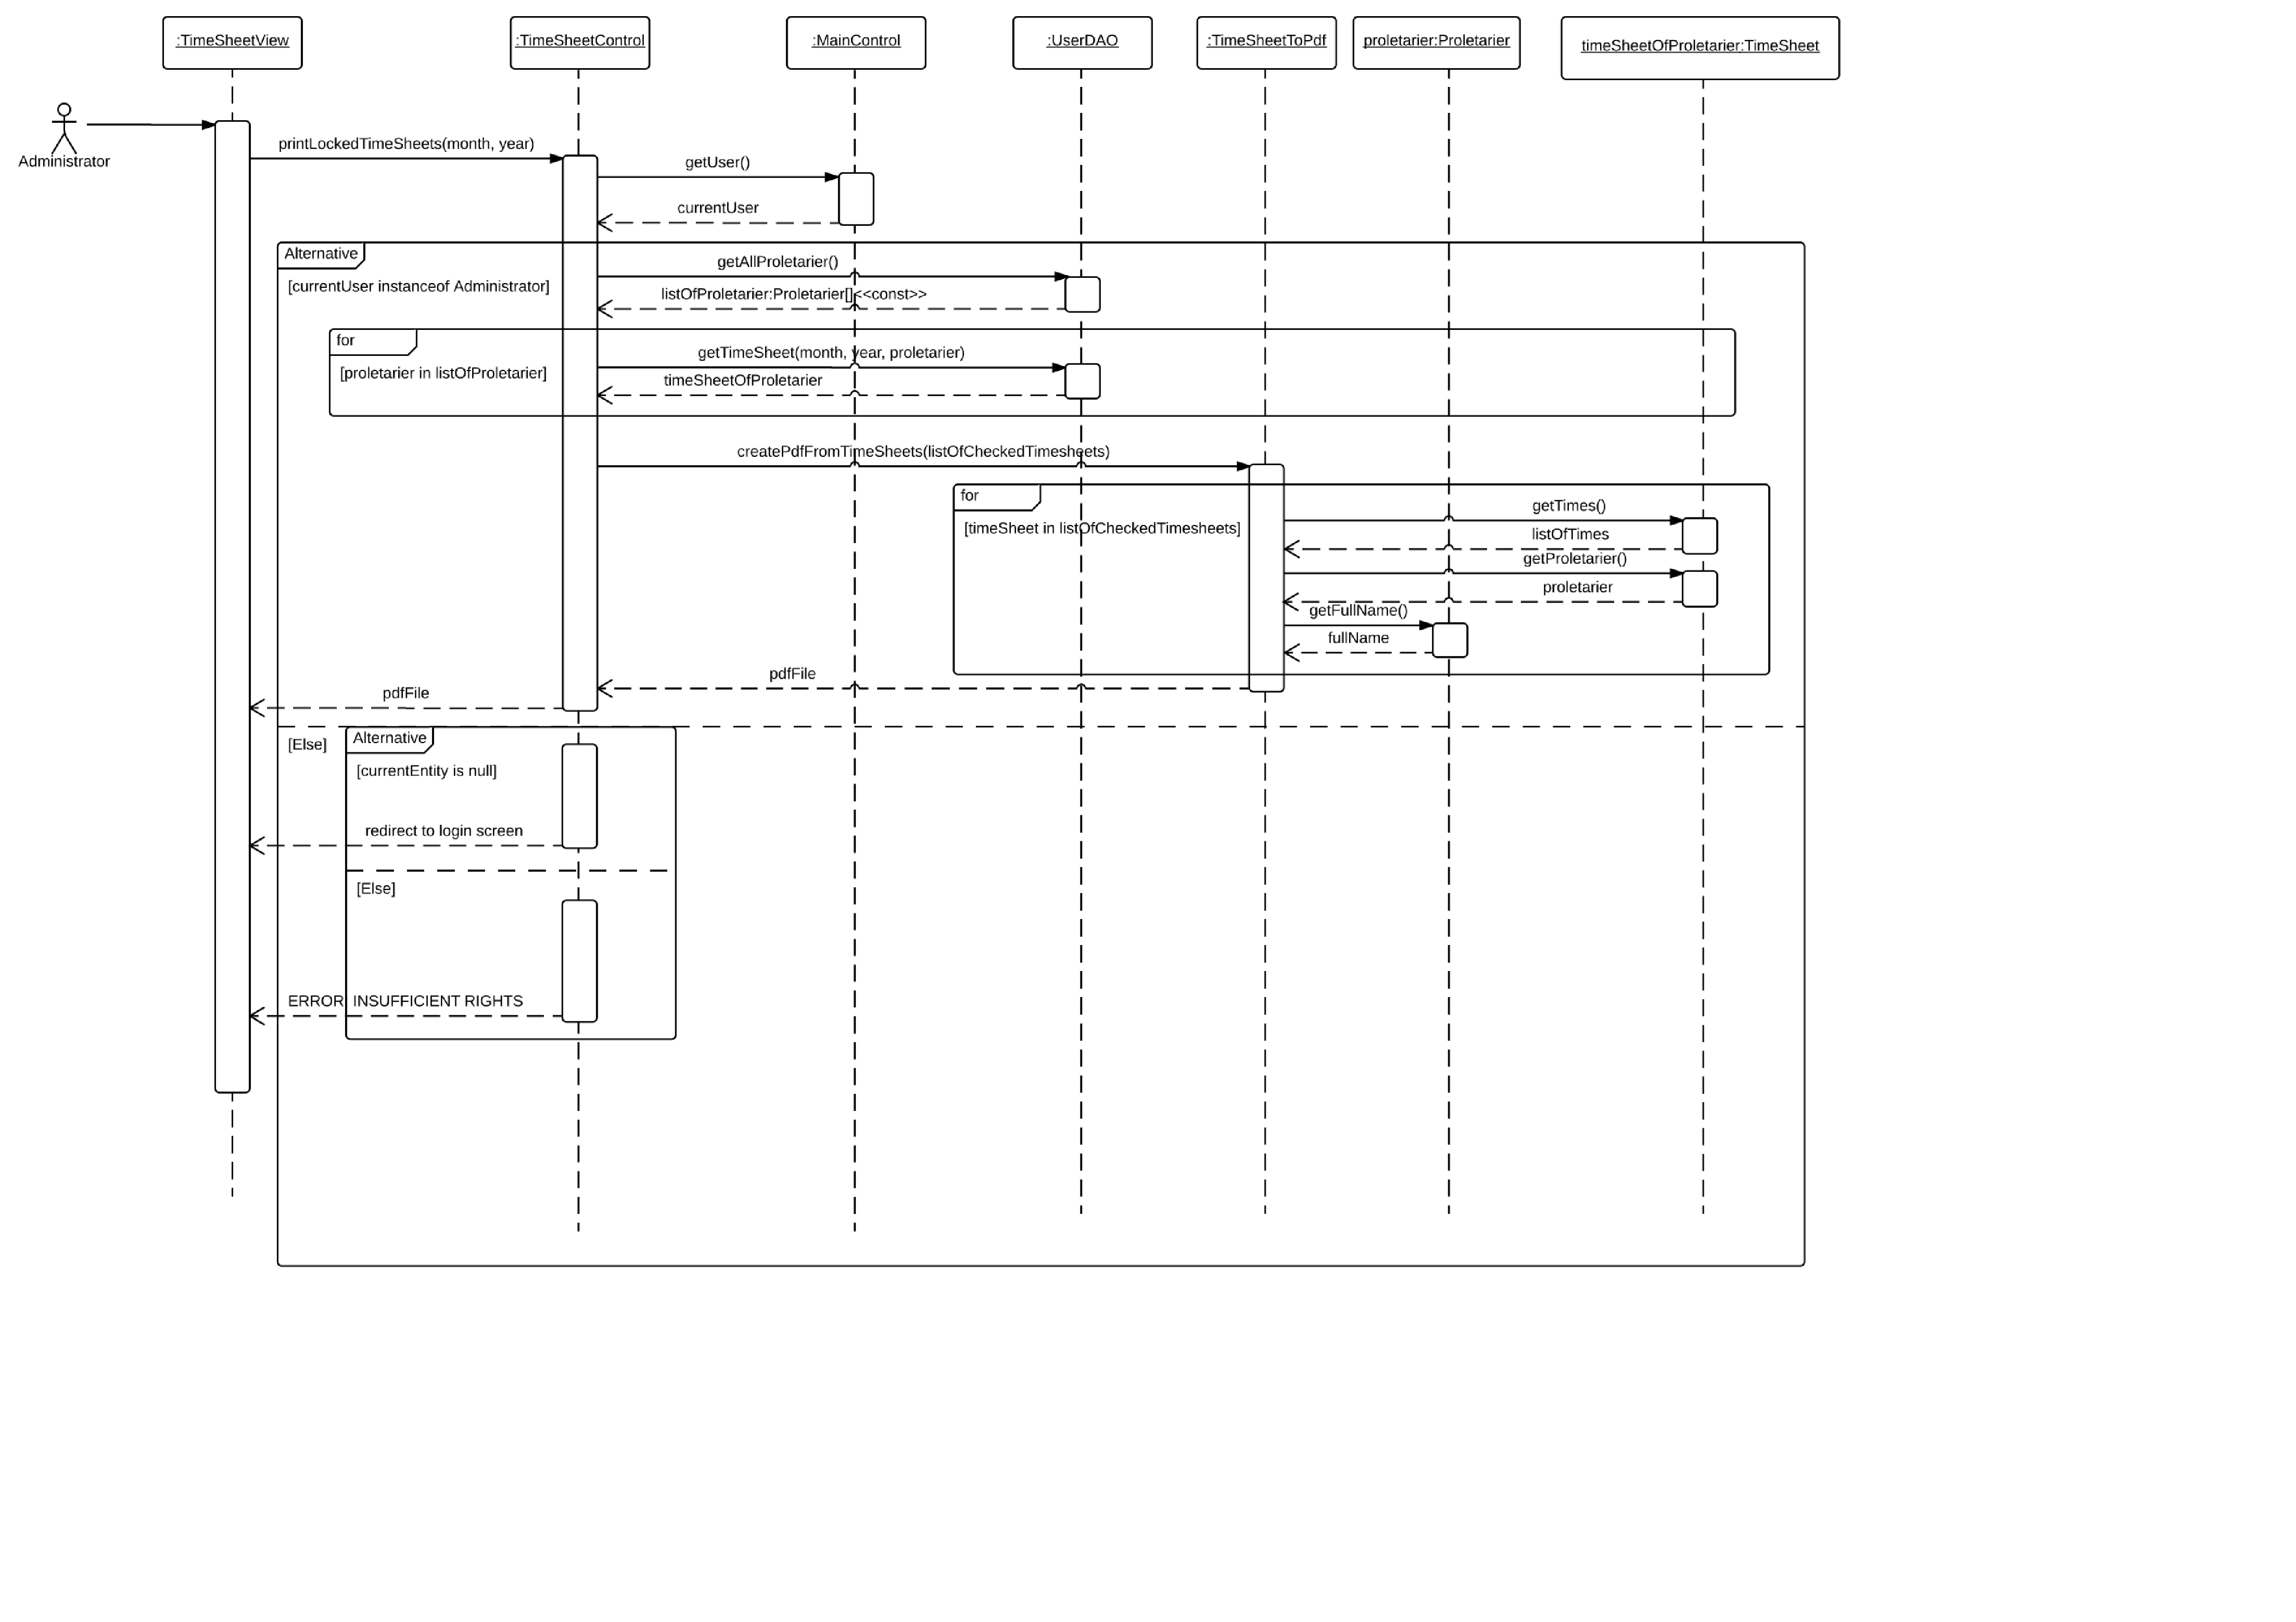
\includegraphics[scale=0.1]{Admin-prints-all-timesheets.pdf}
       \caption{Alte Admin druckt Sequenz}
    \end{figure}

    \paragraph{Veränderungen}
    \begin{itemize}
        \item Der Ablauf durch Hibernate stark vereinfacht
        \begin{itemize}
            \item Anstatt durch die for Schleifen die Stundezettel iterativ zu sammeln, genügt nun eine SQL abfrage im DAO um alle Stundenzettel zu erhalten
        \end{itemize}
        \item Das drucken übernimmt nun eine Subfunktion des TimeSheetHandlers
    \end{itemize}

    \begin{figure}[H]
      \centering
        %\includegraphics[scale=0.1]{}
       \caption{Aufgrund der Vereinfachungen durch hibernate ist ein Sequenzdiagramm hier nicht notwendig}
    \end{figure}


    \newpage
    \subsubsection{Alle Stundenzettel von Nutzer eines Supervisor einholen - Sequenz}

        Wird in der derzeitigen Implementierung nicht benötigt, ist deshalb auch nicht implementiert
        \begin{figure}[H]
          \centering
            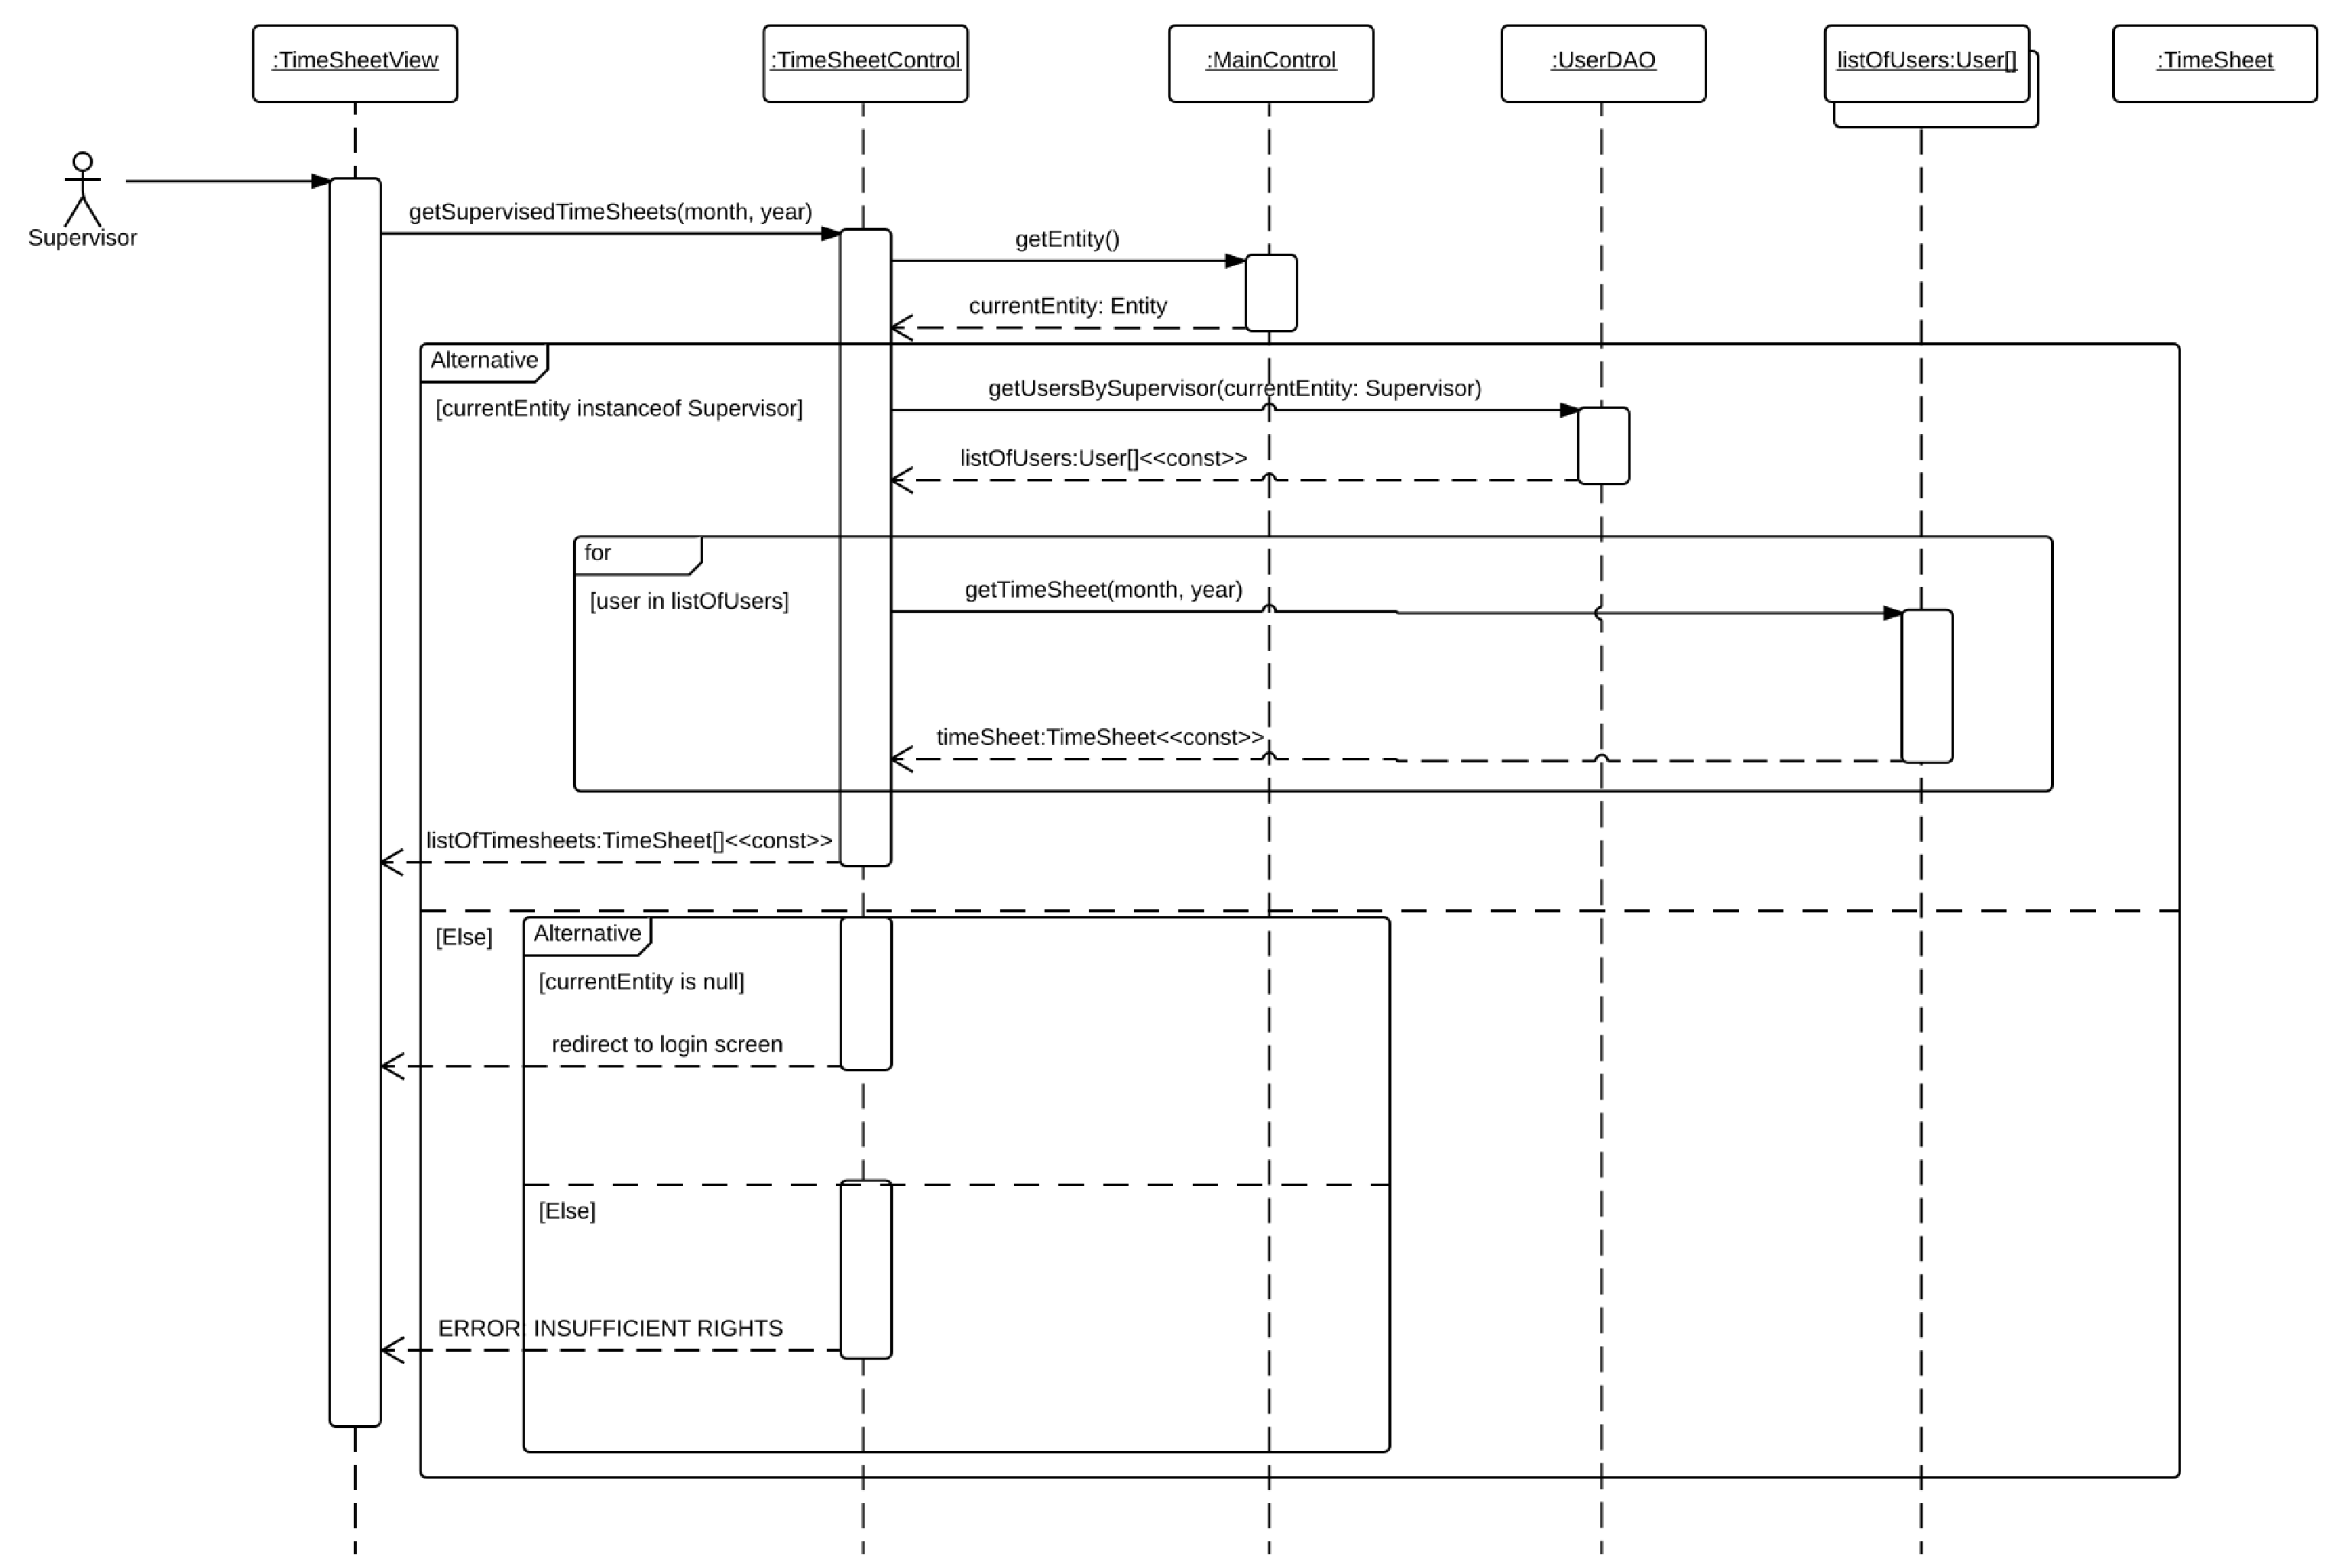
\includegraphics[scale=0.1]{Get-timesheets-of-all-supervised-users.pdf}
           \caption{Alte Admin druckt Sequenz}
        \end{figure}

        \paragraph{Veränderungen}
        \begin{itemize}
            \item Der Ablauf wäre durch Hibernate stark vereinfacht
            \begin{itemize}
                \item Anstatt durch die for Schleifen die Stundezettel iterativ zu sammeln, genügt nun eine SQL abfrage im DAO um alle Stundenzettel zu erhalten
            \end{itemize}
        \end{itemize}

        \begin{figure}[H]
          \centering
            %\includegraphics[scale=0.1]{}
           \caption{Aufgrund der Vereinfachungen durch hibernate ist ein Sequenzdiagramm hier nicht notwendig}
        \end{figure}

    \newpage
        \subsubsection{Nachrichten Versenden und Empfangem - Sequenz}

            \begin{figure}[H]
              \centering
                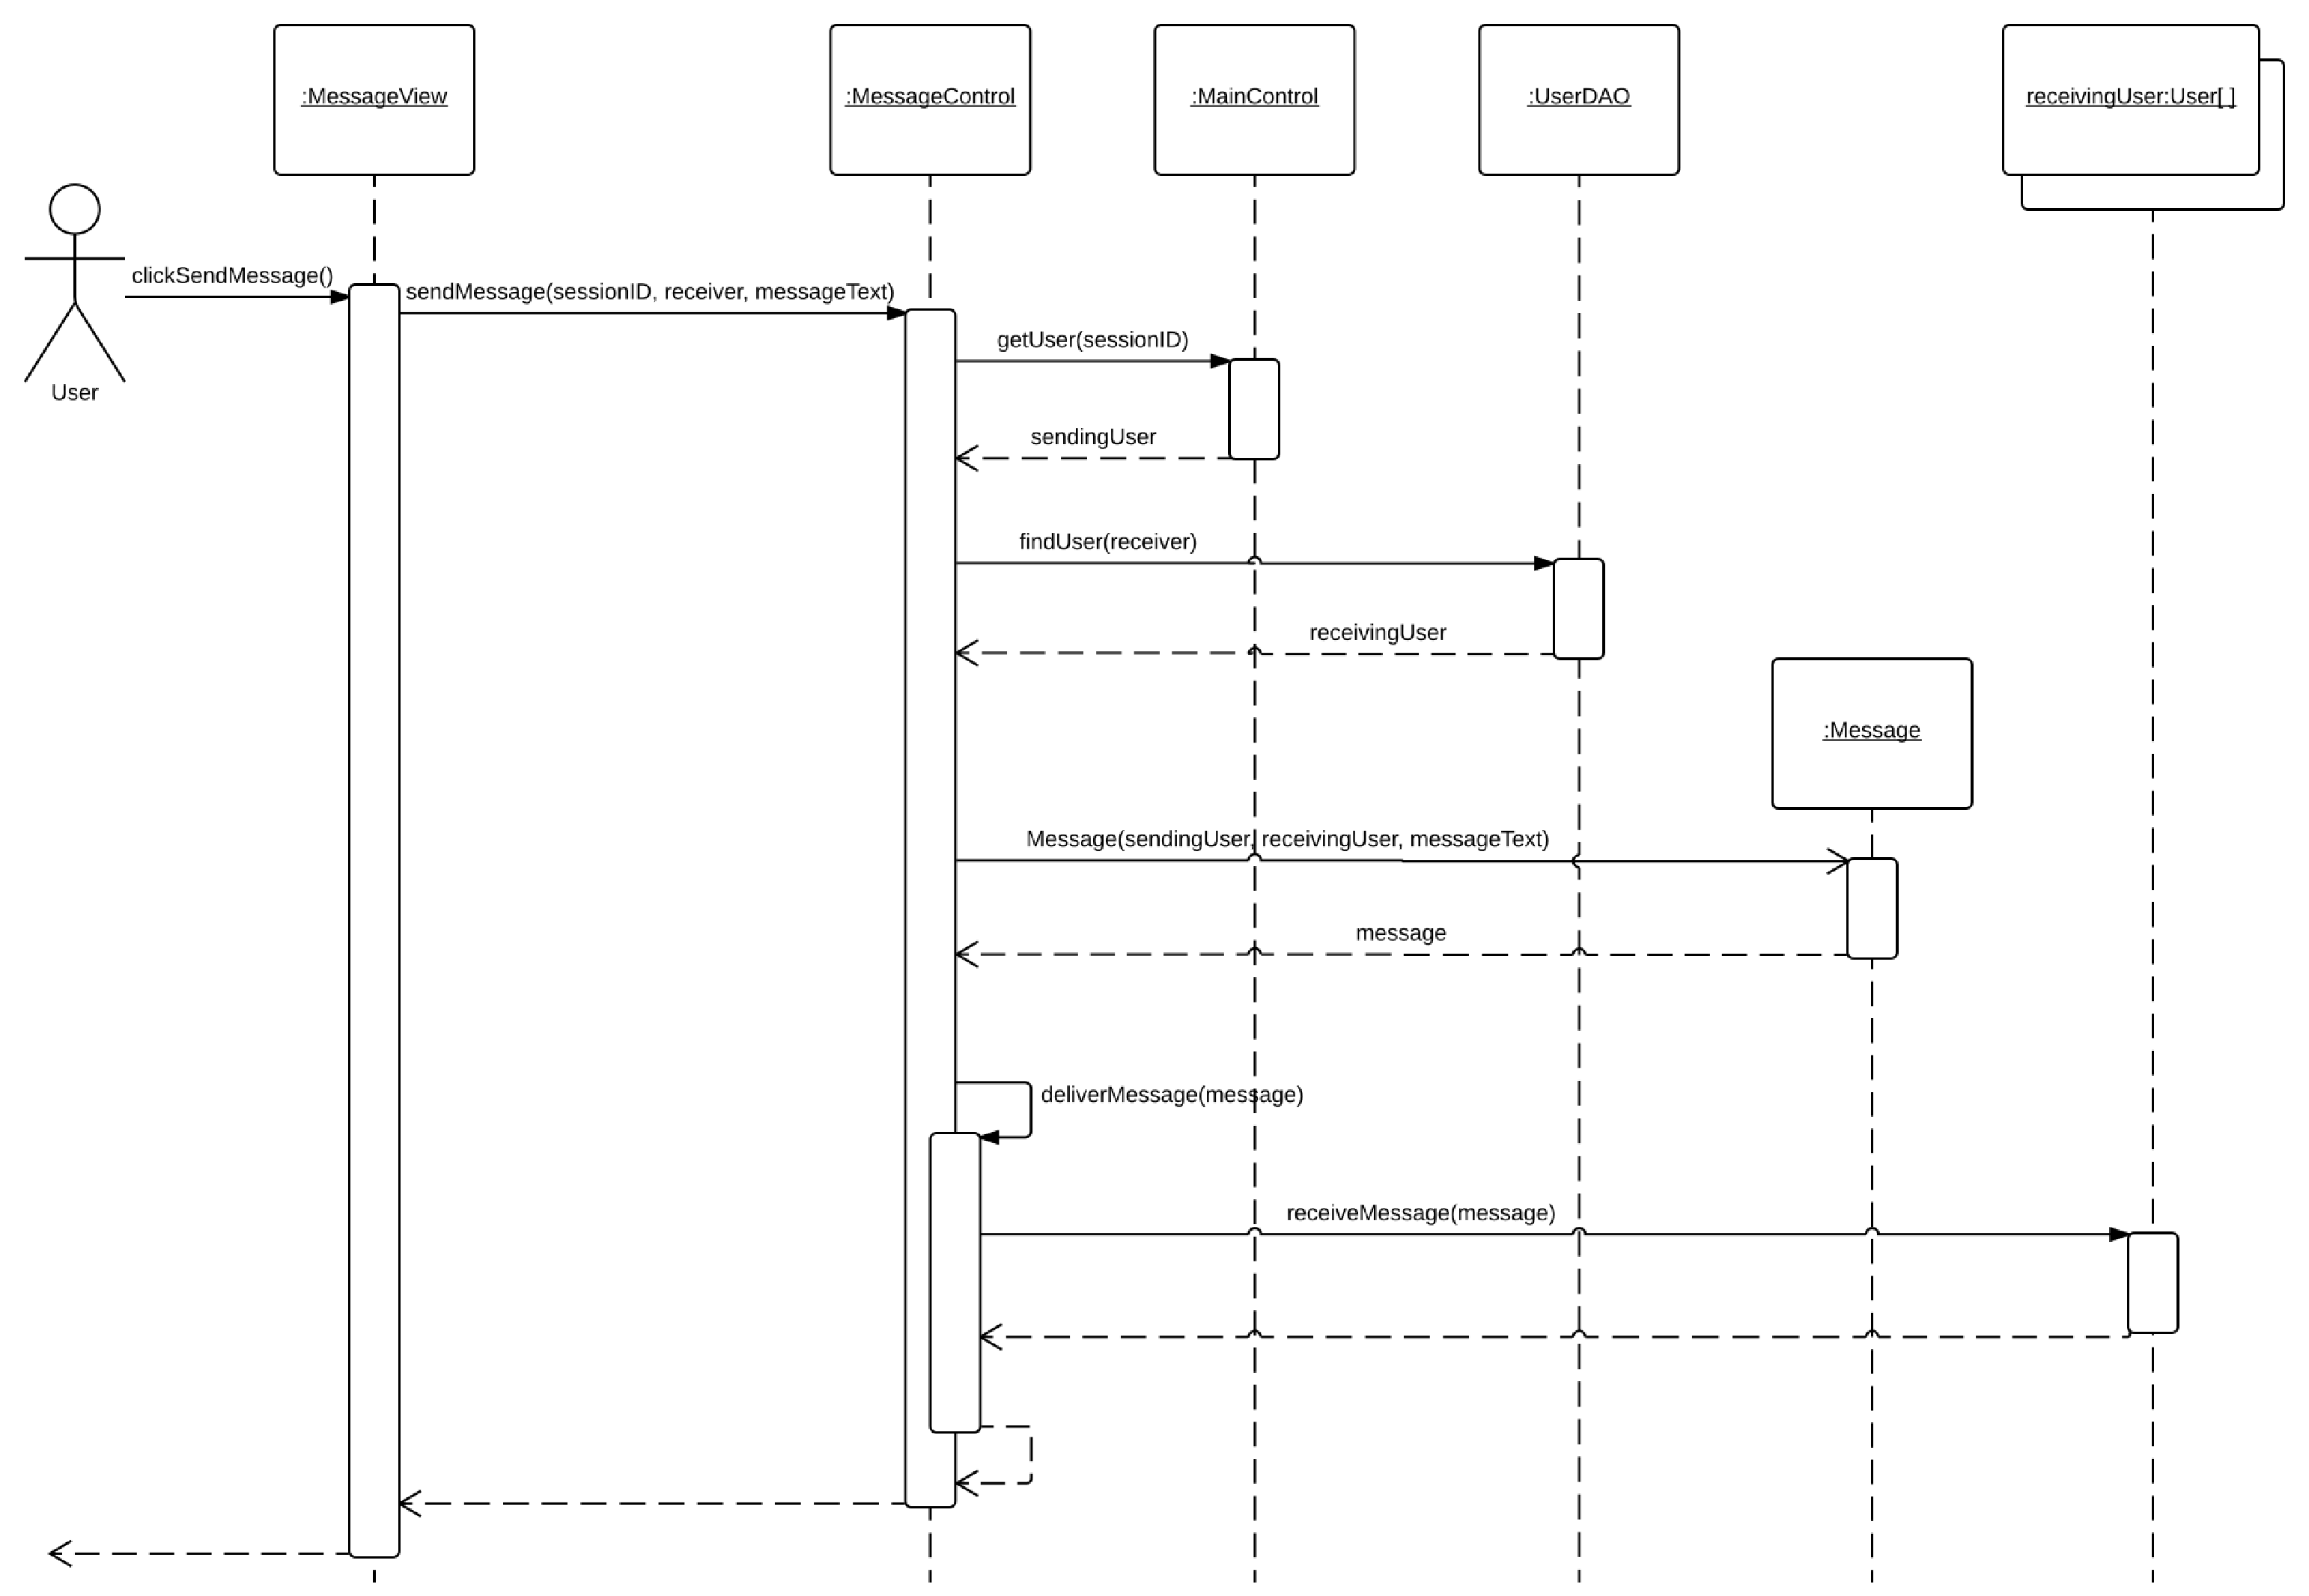
\includegraphics[scale=0.1]{Message-Delivery.pdf}
               \caption{alte Message Delivery Sequenz}
            \end{figure}

            \paragraph{Veränderungen}
                Durch sich veränderte Anforderungen wurde das komplette Message Delivery System obsolet.
            \begin{figure}[H]
              \centering
                %\includegraphics[scale=0.1]{}
               \caption{Da nichtmehr vorhanden keine neue Version verfügbar}
            \end{figure}


    \newpage
        \subsubsection{Holen des derzeitigen Timesheets - Sequenz}
            \begin{figure}[H]
              \centering
                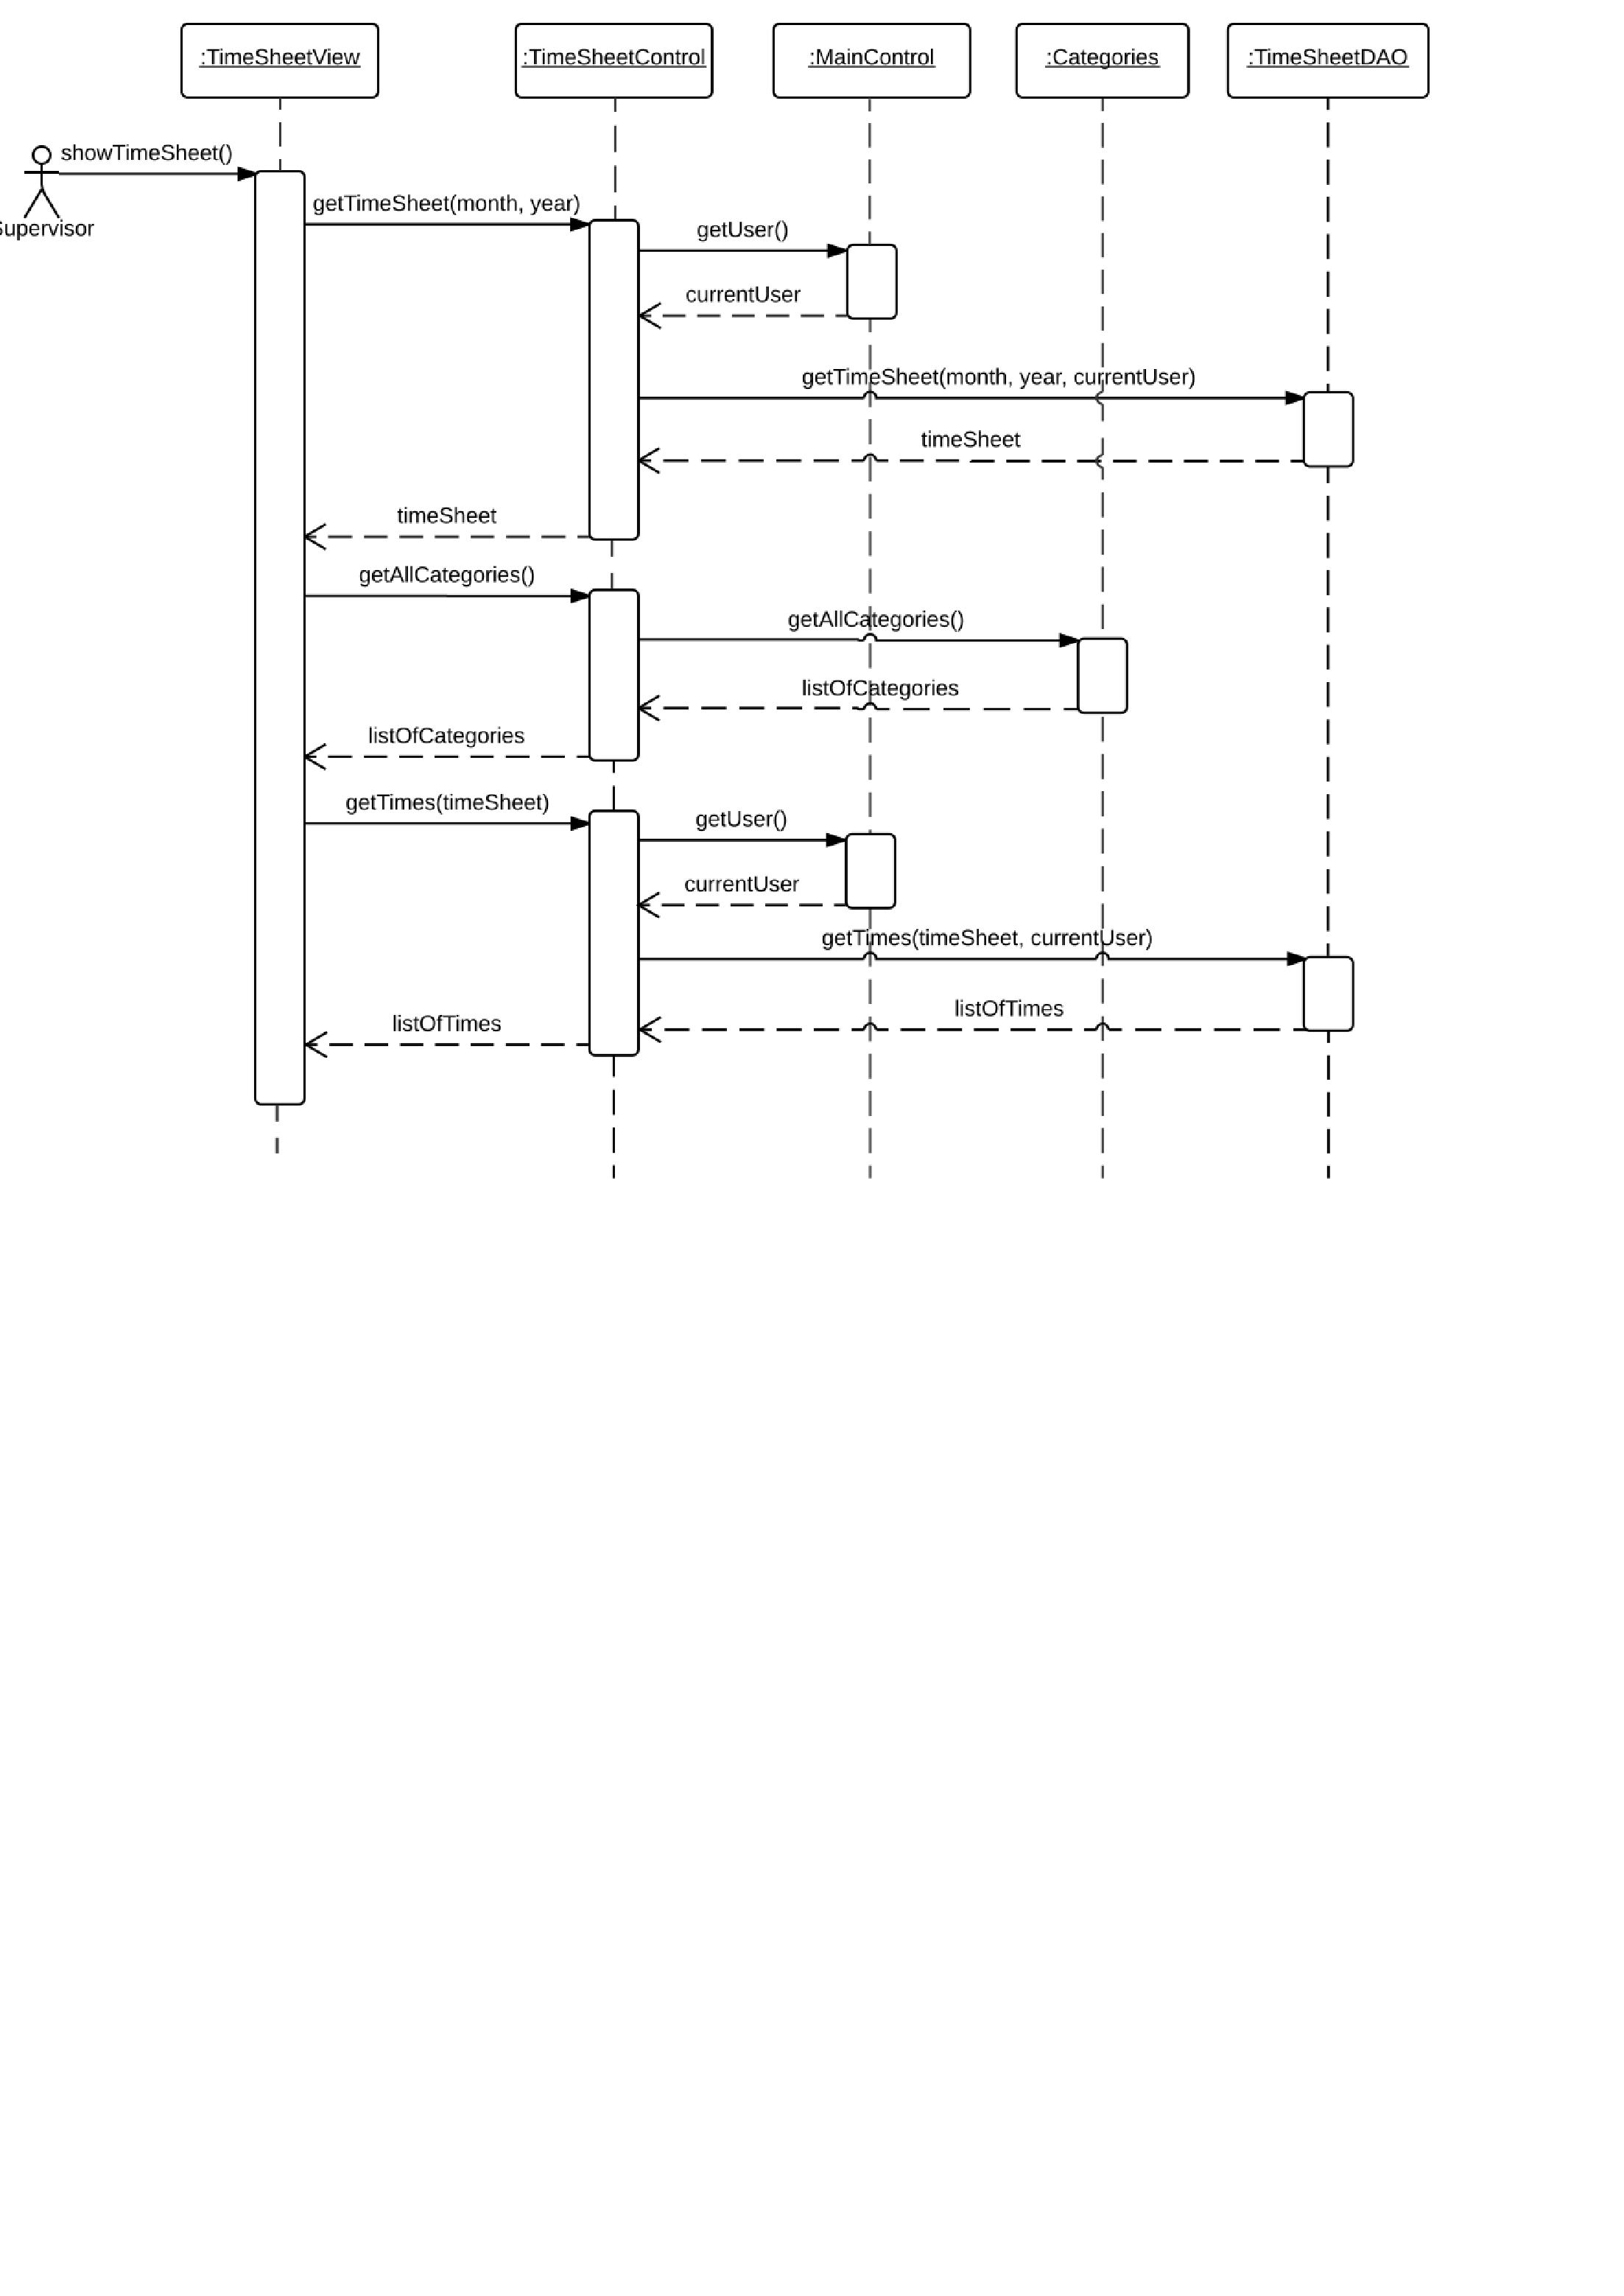
\includegraphics[scale=0.1]{Get-current-timesheet.pdf}
               \caption{altes Holen des aktuellen timeSheets Sequenz}
            \end{figure}

            \paragraph{Veränderungen}
                Es wird nurnoch ein timeSheet Objekt zur View durchgereicht.
                Diese arbeitet dann intern mit den im Objekt vorhandenen Daten
            \begin{figure}[H]
              \centering
                %\includegraphics[scale=0.1]{}
               \caption{Keine neue Sequenz notwendig, da stark vereinfacht}
            \end{figure}

    \newpage
        \subsubsection{Einsenden eines Studenzettels - Sequenz}
                    \begin{figure}[H]
                      \centering
                        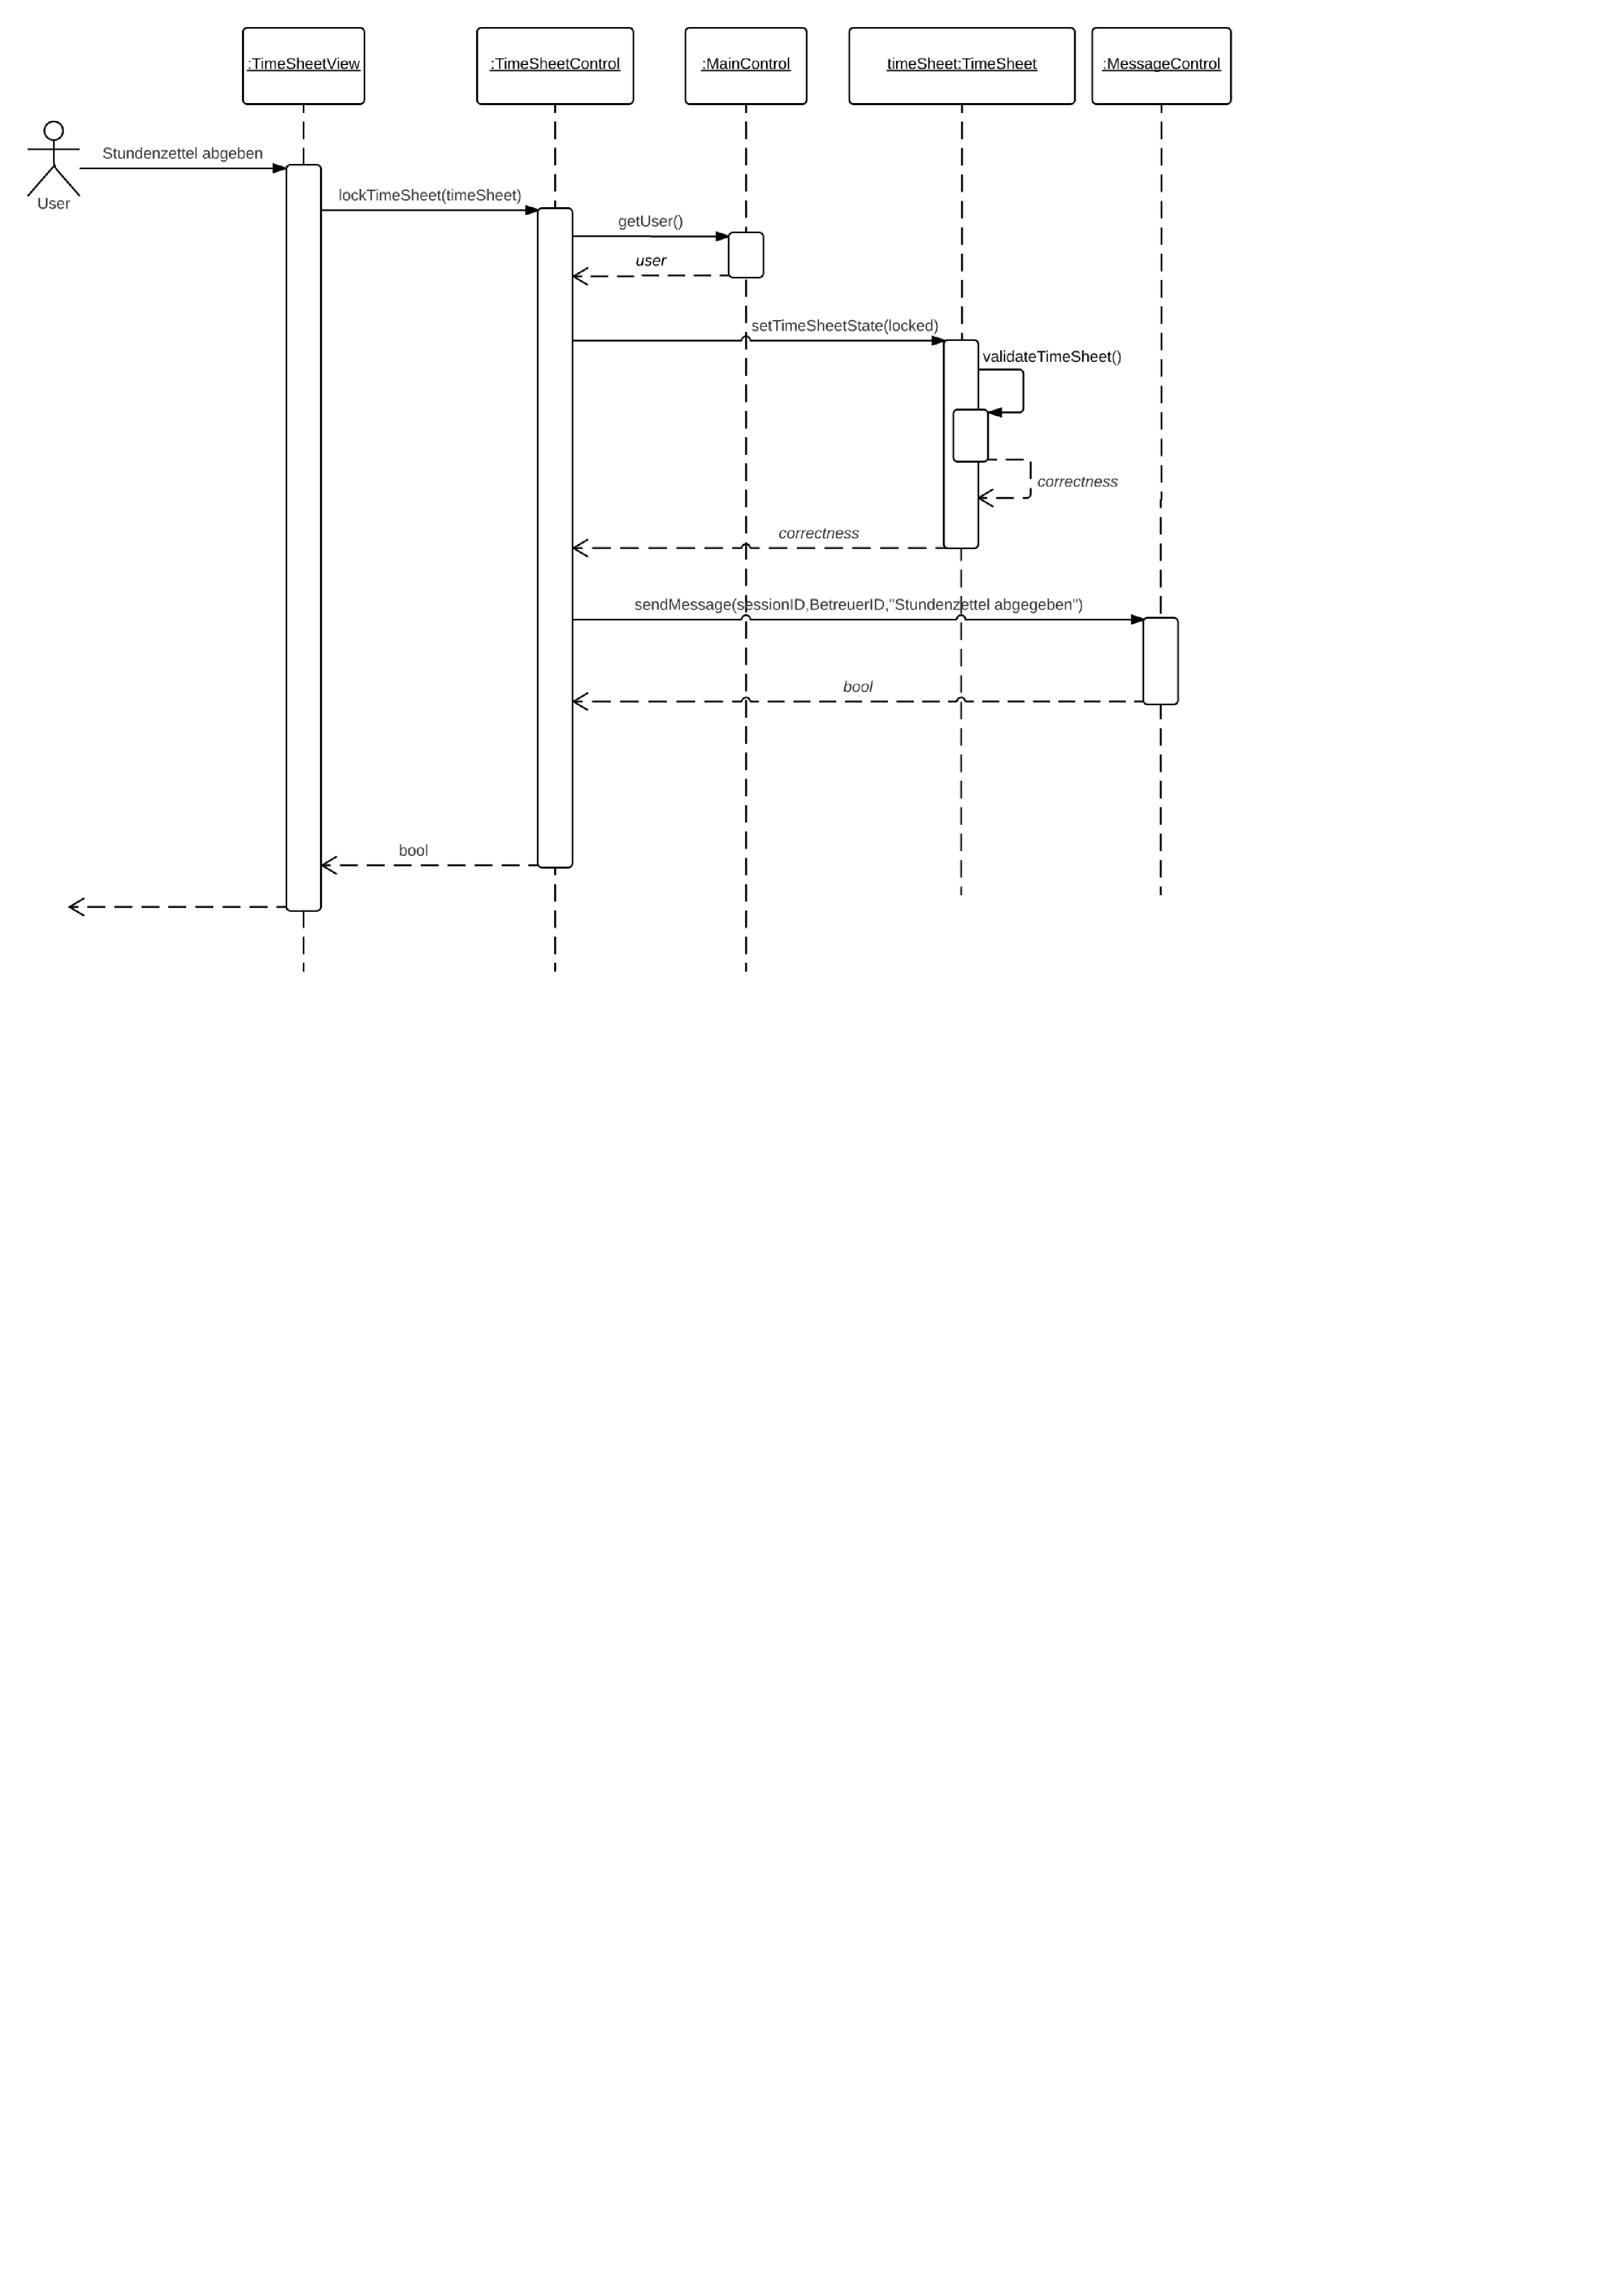
\includegraphics[scale=0.1]{send-in-timesheet.pdf}
                       \caption{altes einsenden eines fertigen Stundenzettels  Sequenz}
                    \end{figure}

                    \paragraph{Veränderungen}
                    \begin{itemize}
                        \item Keine Benachrichtugungen mehr, da keine interne Nachrichten struktur
                        \item Benachrichtigung wird per EMail versendet
                        \item Das Einsenden wurde mit den \emph{locken} eines TimeSheets vereinfacht
                    \end{itemize}
                    \begin{figure}[H]
                      \centering
                        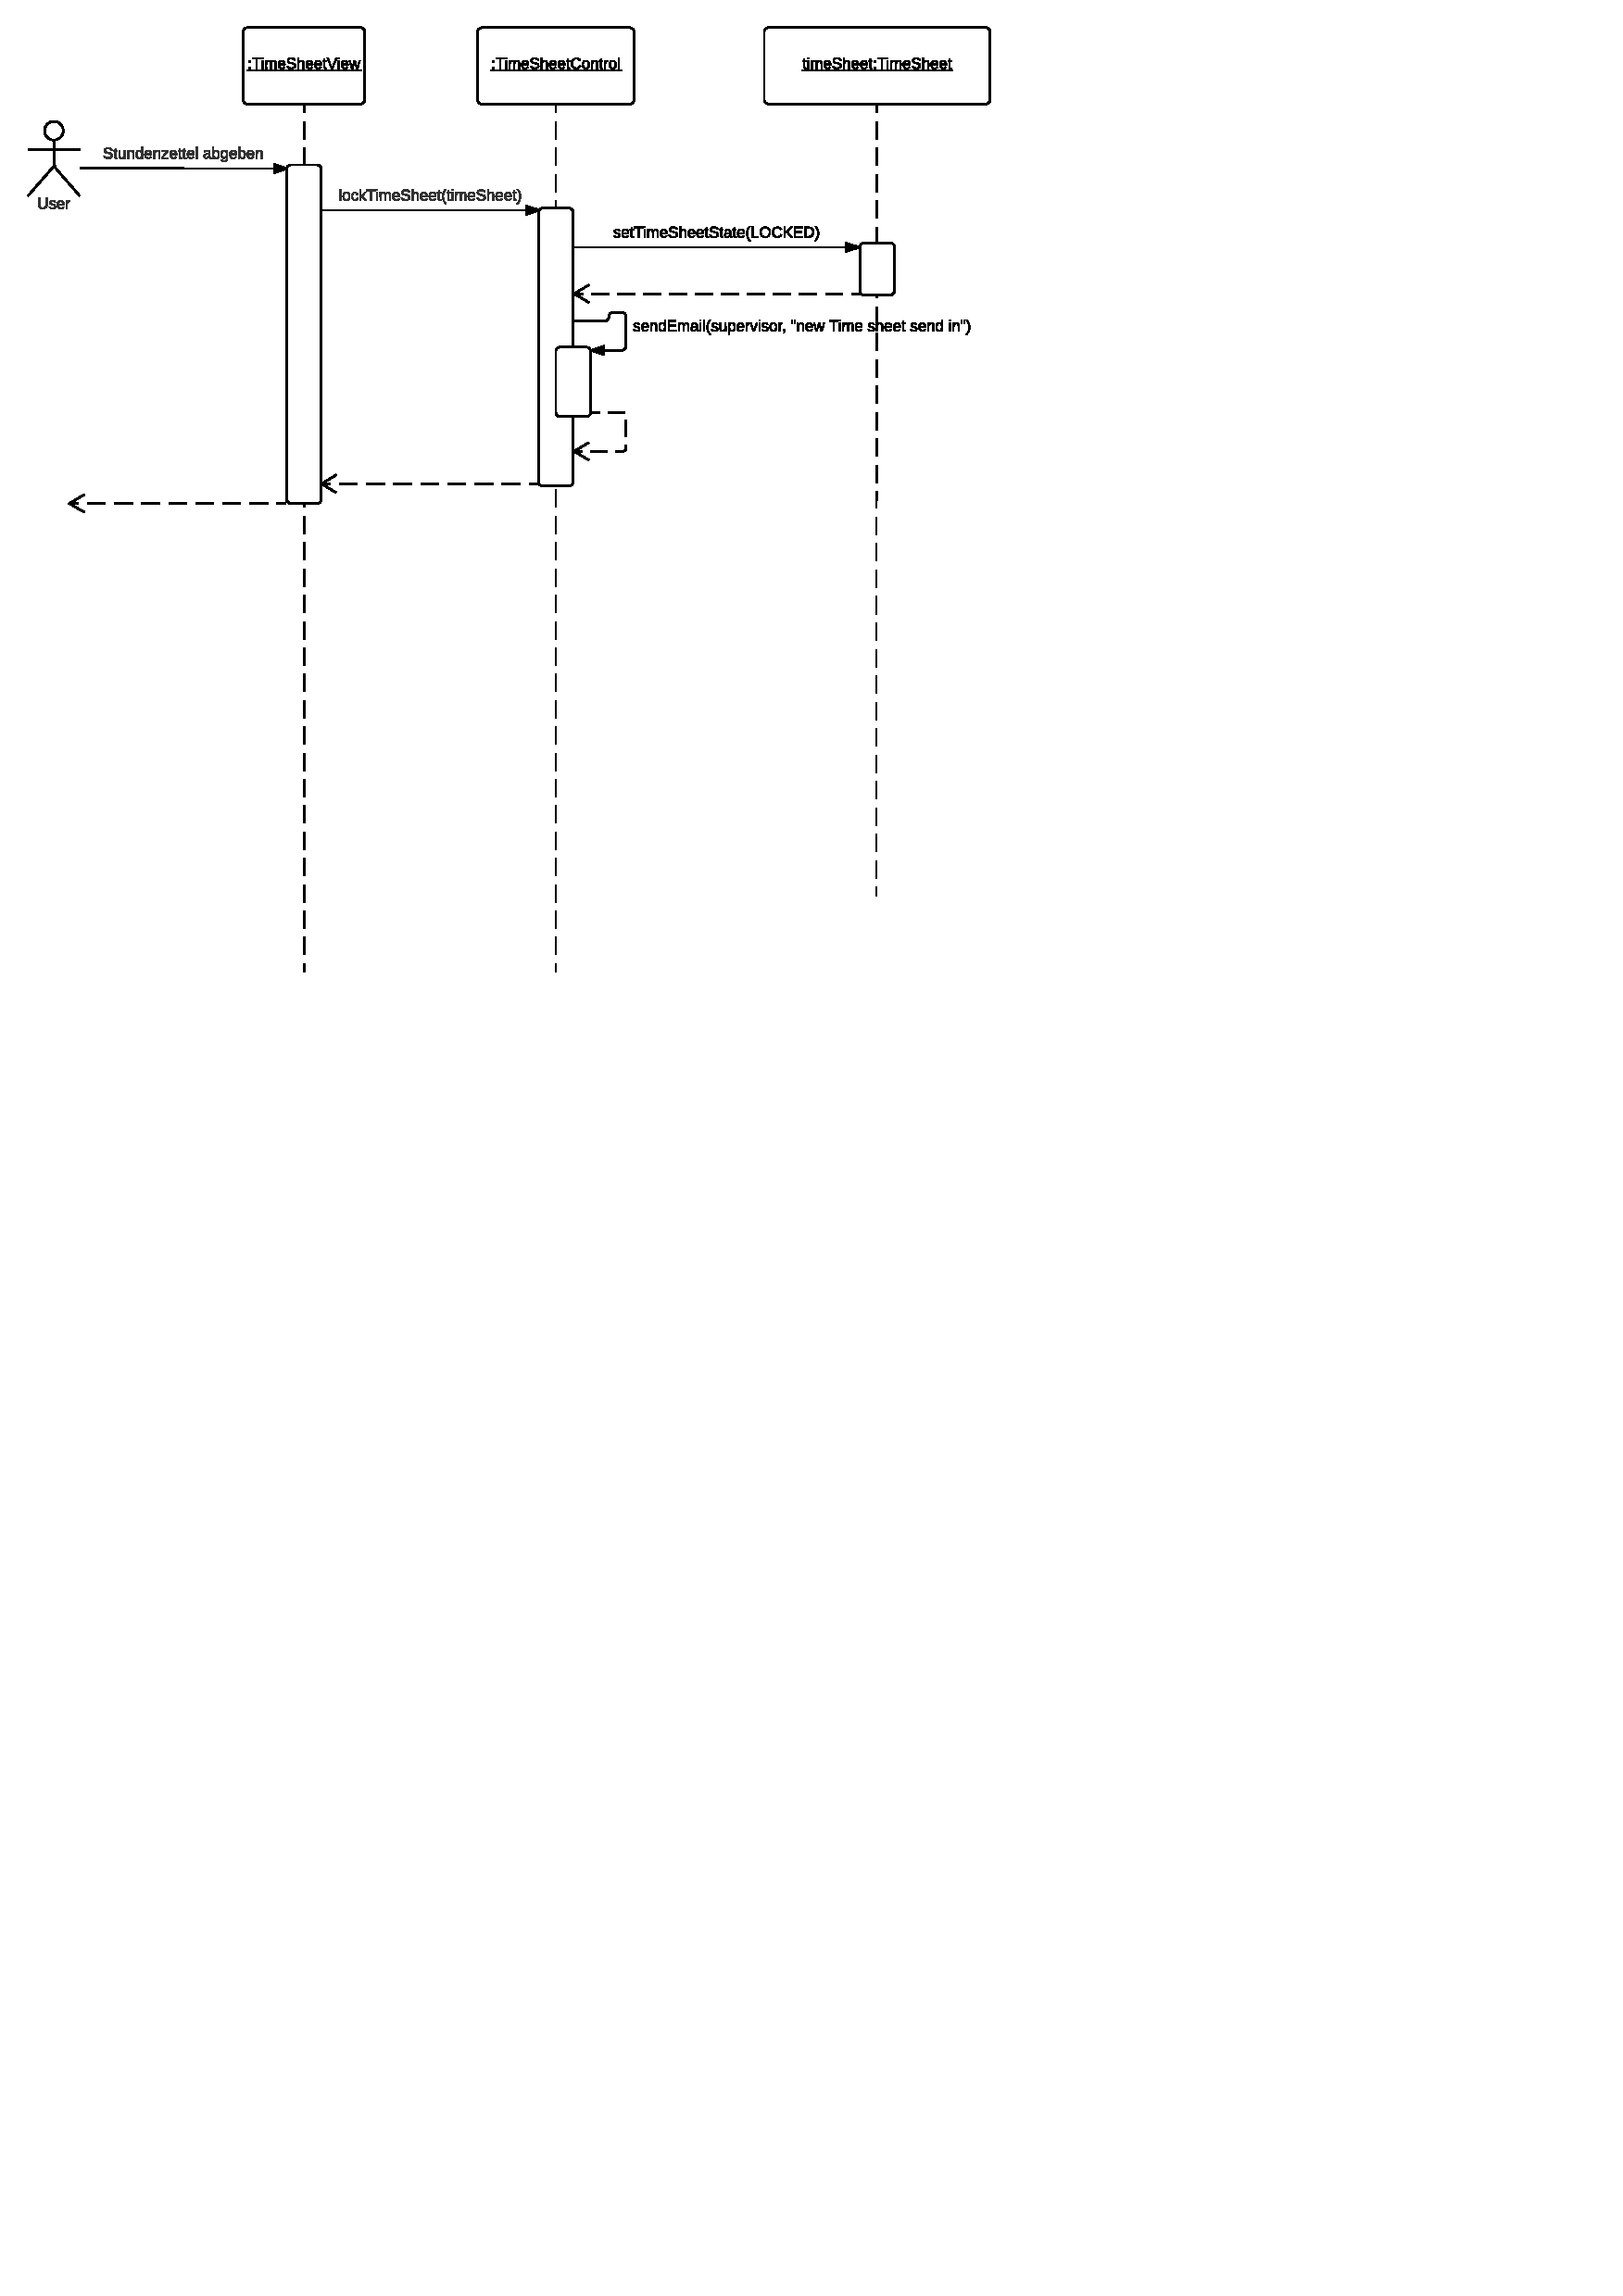
\includegraphics[scale=0.1]{send-in-timesheet-new.pdf}
                       \caption{neues Einsenden von Stundenzetteln}
                    \end{figure}
